% -*-memoria.tex-*-
% Este fichero es parte de la plantilla LaTeX para
% la realización de Proyectos Final de Carrera, protejido
% bajo los términos de la licencia GFDL.
% Para más información, la licencia completa viene incluida en el
% fichero fdl-1.3.tex

% Copyright (C) 2009 Pablo Recio Quijano 

%-------------------------------------------------------
% ---- Plantilla para libros / memorias PFC -----

% Realizada por Pablo Recio Quijano y Noelia Sales Montes 
% Formato de portada y primera página tomado del PFC de
% Francisco Javier Vázquez Púa, en su proyecto 'libgann'
% -------------------------------------------------------

\documentclass[a4paper,11pt]{book}

\usepackage{./estilos/estiloBase} % Basicamente son todas las
                                  % librerias usadas. En caso de que
                                  % falten librerias se van añadiendo
                                  % al fichero.
\usepackage{./estilos/colores}  % Algunos colores ya generados, para
                                % los algunos estilos más avanzados.
\usepackage{./estilos/comandos} % Algunos comandos personalizados

\graphicspath{{./imagenes/}} % Indicamos la ruta donde se encuentran
                             % las imagenes, para ahorrarnos la ruta
                             % completa, y solo modificar aquí si en
                             % un momento dado lo movemos

\begin{document}

% Renombramos las figuras y las tablas
\renewcommand{\figurename}{Figura}
\renewcommand{\listfigurename}{Indice de figuras}
\renewcommand{\tablename}{Tabla}
\renewcommand{\listtablename}{Indice de tablas}

\pagestyle{empty}
% -*-portada.tex-*-
% Este fichero es parte de la plantilla LaTeX para
% la realización de Proyectos Final de Carrera, protejido
% bajo los términos de la licencia GFDL.
% Para más información, la licencia completa viene incluida en el
% fichero fdl-1.3.tex

% Fuente tomada del PFC 'libgann' de Javier Vázquez Púa

\begin{titlepage}

  \begin{center}

    
\includegraphics[scale=0.2]{logo_uca.png} \\
    
    \vspace{2.0cm}
    
    \LARGE{\textbf{ESCUELA SUPERIOR DE INGENIERÍA}} \\
    
    \vspace{1.0cm}
    
    \Large{\textbf{INGENIERÍA TÉCNICA EN INFORMÁTICA DE SISTEMAS}} \\
    
    \vspace{3.0cm}
    
    \Large{SeniorFitness: Aplicación e-health para la valoración de la condición física funcional de personas mayores.} \\
    
    \vspace{2.0cm}
    
    \Large{Álvaro González Álvarez} \\
  
    \vspace{0.5cm}

    \large{\today}
    
  \end{center}
\end{titlepage}

\cleardoublepage

% -*-primerahoja.tex-*-
% Este fichero es parte de la plantilla LaTeX para
% la realización de Proyectos Final de Carrera, protejido
% bajo los términos de la licencia GFDL.
% Para más información, la licencia completa viene incluida en el
% fichero fdl-1.3.tex

% Fuente tomada del PFC 'libgann' de Javier Vázquez Púa

\begin{center}

  
\includegraphics[scale=0.2]{logo_uca.png} \\

  \vspace{2.0cm}

  \Large{ESCUELA SUPERIOR DE INGENIERÍA} \\

  \vspace{1.0cm}

  \large{INGENIERO TÉCNICO EN INFORMÁTICA DE SISTEMAS} \\

  \vspace{2.0cm}

  \large{SeniorFitness: Aplicación e-health para la valoración de la condición física funcional de personas mayores.} \\

  \vspace{1.0cm}

\end{center}

\begin{itemize}
\item \large{Departamento: Lenguajes y sistemas informáticos}
\item \large{Director del proyecto: Raquel Ureña Pérez}
\item \large{Autor del proyecto: Álvaro González Álvarez}
\end{itemize}

\vspace{1.0cm}

\begin{flushright}
  \large{Cádiz, \today} \\

  \vspace{2.5cm}

  \large{Fdo: Álvaro González Álvarez}
\end{flushright}

\cleardoublepage
\pagestyle{plain}

\frontmatter % Introducción, índices ...

% -*-previo.tex-*-
% Este fichero es parte de la plantilla LaTeX para
% la realización de Proyectos Final de Carrera, protejido
% bajo los términos de la licencia GFDL.
% Para más información, la licencia completa viene incluida en el
% fichero fdl-1.3.tex

% Copyright (C) 2009 Pablo Recio Quijano 

\section*{Agradecimientos}

Me gustaria agradecer y/o dedicar este texto a ...

\cleardoublepage

\section*{Licencia} % Por ejemplo GFDL, aunque puede ser cualquiera

Este documento ha sido liberado bajo Licencia GFDL 1.3 (GNU Free
Documentation License). Se incluyen los términos de la licencia en
inglés al final del mismo.\\

Copyright (c) 2017 Álvaro González Álvarez.\\

Permission is granted to copy, distribute and/or modify this document under the
terms of the GNU Free Documentation License, Version 1.3 or any later version
published by the Free Software Foundation; with no Invariant Sections, no
Front-Cover Texts, and no Back-Cover Texts. A copy of the license is included in
the section entitled "GNU Free Documentation License".\\

\cleardoublepage

\section*{Notación y formato}

Aquí incluiremos los aspectos relevantes a la notación y el formato a
lo largo del documento. Para simplificar podemos generar comandos
nuevos que nos ayuden a ello, ver \texttt{comandos.sty} para más
información. 

Cuando nos refiramos a un programa en concreto, utilizaremos la
notación: \\ \programa{emacs}.\\

Cuando nos refiramos a un comando, o función de un lenguaje, usaremos
la notación: \\ \comando{quicksort}.\\

\cleardoublepage

\section*{Resumen}

Es un hecho que el ejercicio físico puede paliar las limitaciones que va imponiendo el proceso de envejecimiento en las personas, pero este debe ser individualizado a las características de la persona mayor, y es por ello que es necesaria la valoración de la condición física de ésta. La Senior Fitness Test (SFT) es una batería de pruebas para tal valoración, y es una de las pocas que está adaptada a los mayores.\\

Esta batería evalúa la condición física funcional, entendiendo por este término: \textit{la capacidad física para desarrollar actividades normales de la vida diaria de forma segura, con independencia y sin una excesiva fatiga} (Rikli y Jones, 2001). Los parámetros de condición física que incluye dicha batería son: fuerza muscular (miembros superiores e inferiores), resistencia aeróbica, flexibilidad (miembros superiores e inferiores) y agilidad.\\

La aplicación Android que se presenta en este documento tiene como empresa darle al usuario la posibilidad de realizar los ejercicios que componen la SFT para cuantas personas mayores el usuario desee registrar en la aplicación, así como almacenar y llevar un control sobre los resultados obtenidos para cada una de ellas. Las numerosas características y sensores de los que disponen actualmente los dispositivos móviles facilitan en gran medida la monitorización de cada uno de los ejercicios y además reducen los materiales necesarios para obtener y registrar los resultados.\\

\textbf{Palabras claves}: Android, Aplicación, Senior Fitness Test, Persona Mayor, Ejercicio Físico

\tableofcontents
\listoffigures
\listoftables

\mainmatter % Contenido en si ...

\chapter{Introducción}
% -*-cap1.tex-*-
% Este fichero es parte de la plantilla LaTeX para
% la realización de Proyectos Final de Carrera, protejido
% bajo los términos de la licencia GFDL.
% Para más información, la licencia completa viene incluida en el
% fichero fdl-1.3.tex

% Copyright (C) 2009 Pablo Recio Quijano 

A continuación, se describe la motivación del presente proyecto y su alcance, y justificaremos la elección de un proyecto como el presente. También se incluye un glosario de términos y la organización del resto de la presente documentación.

\section{Motivación}

Actualmente, si tomamos como referencia la población española, las personas mayores de 65 años representan el 18,4\% del número total de habitantes (INE, 2016) \cite{website:ine}, y se espera que este porcentaje continue aumentando en las próximas décadas. Por tanto, es esperable encontrarnos cada vez con mayor número de personas mayores y a su vez con más limitaciones físicas, que vendrán dadas principalmente por el irreversible proceso de envejecimiento, y muchas de las cuales pueden paliarse con el ejercicio físico. Sin embargo, para conseguir los máximos beneficios del ejercicio para cada persona es de vital relevancia conocer la condición física del mayor para la correcta prescripción de ejercicio, y es en este punto donde entra en juego la Senior Fitness Test (SFT), una batería de pruebas específicamente diseñada para evaluar la condición física funcional de las personas mayores.\\

Partiendo de esta base y teniendo en cuenta que actualmente es cada vez más frecuente el uso de dispositivos móviles por una amplia gama de usuarios y que el rango de edad de los mismos crece sin detenerse, se determinó que sería interesante desarrollar una aplicación móvil que, con la ayuda de los numerosos sensores de los que disponen los dispositivos móviles de hoy en día, sirviese como herramienta para realizar las diferentes pruebas físicas que componen la SFT, y además diese la posibilidad de registrar y consultar los resultados obtenidos para cada sujeto en las diferentes sesiones realizadas.\\

De esta forma cualquier profesional dentro del sector de Ciencias de la Salud, de la Actividad Física o del Deporte que esté interesado en llevar un seguimiento de la condición física funcional de personas mayores, puede hacer uso de la aplicación para que ésta contabilice de forma autónoma (sin necesidad de tener que contar a ojo ni con la ayuda de un cronómetro) las repeticiones realizadas y los tiempos obtenidos por los sujetos para cada uno de los diferentes ejercicios de la batería de pruebas, además de quedar registrados en el perfil de cada persona para su estudio.\\

Debido a todo lo anteriormente mencionado y a que el aprendizaje de las tecnologías empleadas resulta muy útil de cara al mercado laboral por tratarse de tecnologías punteras en la actualidad, puede justificarse un proyecto como el presente como Proyecto de Fin de Carrera.

\section{Alcance}

El alcance del proyecto consiste en la realización de una aplicación Android que, mediante los sensores que contienen los dispositivos móviles actuales tales como el acelerómetro, el giroscopio o el sensor de gravedad, sea capaz de detectar la correcta realización de los ejercicios en los que consiste la SFT.\\

Para que los sensores del dispositivo móvil sean capaces de realizar las lecturas necesarias para el correcto cálculo del movimiento realizado durante la ejecución del ejercicio, es necesario que el usuario siga las instrucciones dadas por la aplicación para cada uno de los diferentes ejercicios físicos. Por ejemplo, puede ser necesario que el dispositivo móvil se coloque en la extremidad (brazo o pierna) con la que se realizará la actividad.\\

Durante la realización de las pruebas que hagan uso de los sensores comentados, el dispositivo móvil dará feedback sobre la correcta realización de los ejercicios, emitiendo un sonido con cada repetición realizada de forma satisfactoria y en el mismo instante en el que se contabiliza, sin que sea necesario observar la pantalla del dispositivo para conocer si se ha realizado adecuadamente el ejercicio.\\

Una vez finalizado cualquiera de los tests, la aplicación da la posibilidad de almacenar el resultado para la persona mayor que esté realizando la batería de pruebas, dándose por concluida la sesión cuando se haya completado el último test que quede pendiente de realizar de la SFT.\\

El usuario puede consultar en todo momento los resultados obtenidos por cada uno de los sujetos que han ido realizando las pruebas, tanto para la sesión que esté en progreso (con algún test pendiente de finalizar) como para aquellas sesiones que ya se completaron con anterioridad, para las cuales se mostrarán las correspondientes estadísticas.\\

La aplicación es de código libre bajo la licencia GNU GPL así como las técnicas y herramientas empleadas para su desarrollo. Su uso será en dispositivos móviles Android.

\section{Glosario de términos}

Esta sección contiene una lista ordenada alfabéticamente de los principales términos, acrónimos y abreviaturas específicos del dominio del problema:

\begin{itemize}
\item \textbf{Android}: Android es un sistema operativo basado en el núcleo Linux. Fue diseñado principalmente para dispositivos móviles con pantalla táctil, como teléfonos inteligentes, tablets y también para relojes inteligentes, televisores y automóviles.
\item \textbf{API}: La interfaz de programación de aplicaciones es un conjunto de subrutinas, funciones y procedimientos (o métodos, en la programación orientada a objetos) que ofrece cierta biblioteca para ser utilizado por otro software como una capa de abstracción.
\item \textbf{APK}: Un archivo con extensión .apk (Android Application Package, significado en español: Aplicación empaquetada de Android) es un paquete para el sistema operativo Android. Este formato es una variante del formato JAR de Java y se usa para distribuir e instalar componentes empaquetados para la plataforma Android.
\item \textbf{Aplicación}: Es un tipo de programa informático diseñado como herramienta para permitir a un usuario realizar uno o diversos tipos de trabajos.
\item \textbf{Condición física funcional}: Capacidad física para desarrollar actividades normales de la vida diaria de forma segura, con independencia y sin una excesiva fatiga (Rikli y Jones, 2001).
\item \textbf{e-health} / \textbf{eHealth} / \textbf{eSalud}: Es el término con el que se define al conjunto de Tecnologías de la Información y la Comunicación (TICs) que, a modo de herramientas, se emplean en el entorno sanitario en materia de prevención, diagnóstico, tratamiento, seguimiento, así como en la gestión de la salud, ahorrando costes al sistema sanitario y mejorando la eficacia de este.
\item \textbf{Framework}: Es un conjunto estandarizado de conceptos, prácticas y criterios para enfocar un tipo de problemática particular que sirve como referencia, para enfrentar y resolver nuevos problemas de índole similar. Un framework proporciona bibliotecas para acceder a bases de datos, estructuras para plantillas y gestión de sesiones, y con frecuencia facilitan la reutilización de código.
\item \textbf{Git}: Es un software de control de versiones diseñado por Linus Torvalds, pensando en la eficiencia y la confiabilidad del mantenimiento de versiones de aplicaciones cuando éstas tienen un gran número de archivos de código fuente.
\item \textbf{GPL}: La Licencia Pública General de GNU es la licencia de derecho de autor más ampliamente usada en el mundo del software y garantiza a los usuarios finales (personas, organizaciones, compañías) la libertad de usar, estudiar, compartir (copiar) y modificar el software.
\item \textbf{IDE}: Un entorno de desarrollo integrado es una aplicación informática que proporciona servicios integrales para facilitarle al desarrollador o programador el desarrollo de software.
\item \textbf{INE}: El Instituto Nacional de Estadística (INE) es un organismo autónomo de España encargado de la coordinación general de los servicios estadísticos de la Administración General del Estado y la vigilancia, control y supervisión de los procedimientos técnicos de los mismos. Entre los trabajos que realiza, destacan las estadísticas sobre la demografía, economía, y sociedad españolas.
\item \textbf{JAR}: Es un tipo de archivo que permite ejecutar aplicaciones escritas en el lenguaje Java.
\item \textbf{Java}: Java es un lenguaje de programación de propósito general, concurrente, orientado a objetos que fue diseñado específicamente para tener tan pocas dependencias de implementación como fuera posible.
\item \textbf{Prueba} /  \textbf{ Test de valoración de la condición física}: Son las pruebas que se realizan con la finalidad de medir y valorar las diferentes cualidades físicas básicas en sus diferentes facetas. La medición y valoración de estas cualidades nos informa del estado actual del sujeto. Este dato es fundamental para la programación del entrenamiento, ya que nos indica si hay que trabajar de forma específica alguna de ellas, en función de los objetivos a alcanzar, o por el contrario hay que trabajar de forma general.
\item \textbf{Repositorio}: Es un sitio centralizado donde se almacena y mantiene información digital, habitualmente bases de datos o archivos informáticos.
\item \textbf{Senior Fitness Test (SFT)}: Es una batería de pruebas de valoración de la condición física diseñada por Rikli y Jones. Surgió por la necesidad de crear una herramienta que nos permitiese valorar la condición física de los mayores con seguridad así como de forma práctica.
\item \textbf{SQL}: Es un lenguaje específico del dominio que da acceso a un sistema de gestión de bases de datos relacionales que permite especificar diversos tipos de operaciones en ellos.
\item \textbf{SQLite}: SQLite es un motor de bases de datos muy popular en la actualidad por ofrecer características tan interesantes como su pequeño tamaño, no necesitar servidor, precisar poca configuración, ser transaccional y ser de código libre. Android incorpora de serie todas las herramientas necesarias para la creación y gestión de bases de datos SQLite, y entre ellas una completa API para llevar a cabo de manera sencilla todas las tareas necesarias.
\item \textbf{UML}: El Lenguaje Unificado de Modelado es el lenguaje de modelado de sistemas de software más conocido y utilizado en la actualidad. Es un lenguaje gráfico para visualizar, especificar, construir y documentar un Sistema.
\item \textbf{XML}: El Lenguaje de Marcas Extensible es un meta-lenguaje que permite definir lenguajes de marcas desarrollado por el World Wide Web Consortium (W3C) utilizado para almacenar datos en forma legible.
\end{itemize}

\section{Organización del Documento}

La estructura del presente documento es la siguiente:

\begin{itemize}
\item \textbf{Introducción}: Apartado introductorio sobre la motivación para desarrollar este proyecto, su alcance, así como la estructuración de este documento.
\item \textbf{Descripción general}: Descripción más amplia sobre el proyecto, así como todas las características relevantes que tendrá.
\item \textbf{Planificación}: En este apartado se detalla la planificación realizada para llevar a cabo el proyecto, así como las distintas etapas en las que está compuesto el mismo.
\item \textbf{Análisis de requisitos}: En este apartado se detallan los objetivos del sistema, requisitos funcionales, requisitos no funcionales, reglas de negocio, requisitos de información y se representará mediante un diagrama inicial el modelo conceptual de datos del proyecto.
\item \textbf{Diseño del sistema}: El diseño del sistema viene dado por una arquitectura general del sistema (tanto física como lógica), patrones de diseño, diseño físico y lógico de datos, el diseño de la interfaz de usuario, diseño del modo de empleo del dispositivo móvil para la detección de movimientos y los diagramas de clases y de secuencia.
\item \textbf{Implementación del sistema}: En este apartado se detallan los aspectos más importantes sobre la implementación del sistema: entorno de construcción y el código fuente.
\item \textbf{Pruebas y validaciones}: Pruebas realizada a la aplicación, con el fin de comprobar su correcto funcionamiento y cumplimiento de las expectativas.
\item \textbf{Conclusiones}: Conclusiones obtenidas sobre el proyecto desarrollado, visión futura del mismo y experiencia adquirida.
\item \textbf{Herramientas utilizadas}: Herramientas software utilizadas a lo largo del desarrollo del proyecto.
\item \textbf{Manual de instalación}: Apartado donde se indica como realizar la instalación de la aplicación en el sistema.
\item \textbf{Manual de usuario}: Manual de usuario para el correcto uso de la aplicación.
\item \textbf{Bibliografía}: Referencias consultadas durante la realización del proyecto.
\item \textbf{Licencia GNU GFDL}: Texto completo sobre la licencia GNU GFDL en inglés.
\end{itemize}



\chapter{Descripción general del proyecto}
% -*-cap2.tex-*-
% Este fichero es parte de la plantilla LaTeX para
% la realización de Proyectos Final de Carrera, protejido
% bajo los términos de la licencia GFDL.
% Para más información, la licencia completa viene incluida en el
% fichero fdl-1.3.tex

% Copyright (C) 2009 Pablo Recio Quijano 

\section{Descripción}

Con la aplicación descrita en el presente documento, el usuario puede registrar en la misma cuantas personas mayores desee. Una vez exista una persona registrada en el sistema, podrá realizar la batería de pruebas de valoración de la condición física en la que consiste la Senior Fitness Test, sirviéndole de ayuda el propio dispositivo móvil donde se encuentre instalada la aplicación.\\

Para ello, dependiendo de la prueba que se haya seleccionado para realizar entre las disponibles, la aplicación hará uso por ejemplo del sensor de gravedad del dispositivo móvil para determinar si el ejercicio se ha realizado de forma satisfactoria (y por tanto contabilizar la repetición), o bien mostrar en pantalla un cronómetro que se deberá usar si la prueba así lo requiere, entre otros casos.\\

Una vez realizada cada prueba para la persona mayor en cuestión, el sistema da la posibilidad de almacenar el resultado obtenido por la aplicación, pudiéndose consultar posteriormente en el historial de sesiones realizadas por dicha persona.

\section{Características de la aplicación}

La aplicación ofrece una alternativa libre y gratuita para poder llevar un registro y control de la condición física funcional de personas mayores, pudiéndose consultar los resultados obtenidos y sus estadísticas asociadas en cualquier lugar y momento. Además, es fácilmente adaptable a nuevos tests o pruebas que se deseen ir incluyendo a la aplicación en un futuro.

\subsection{Componentes de la aplicación}

En esta sección se hará una pequeña descripción de los distintos componentes que conforman la aplicación.

\subsubsection{Usuario}

Usuario de la aplicación, que será quien realice el registro de las personas mayores en el sistema y tenga acceso a las estadísticas y resultados obtenidos para cada una de ellas.

\subsubsection{Personas mayores}

Son los sujetos que se registran en el sistema y quienes realizan las sesiones de ejercicios correspondientes a los tests que componen la batería Senior Fitness Test.

\subsubsection{Tests}

Los tests son las pruebas de valoración de la condición física en las que consiste la batería de pruebas denominada Senior Fitness Test. Los resultados obtenidos en cada uno de los tests se podrán almacenar para la persona mayor que haya realizado el ejercicio.

\subsubsection{Sesiones}

Una sesión es el conjunto de los diferentes tests o pruebas de la batería Senior Fitness Test, y se identifican por el día y la hora en el que se comienza con ella. Se considera que una persona ha completado una sesión cuando ya ha realizado cada uno de los tests de la batería de pruebas y por tanto ha obtenido un resultado para cada una de ellas. En caso de que quede algún test por realizar, la sesión se considera en progreso, y por tanto no se marcará como completada hasta obtener el resultado de las pruebas restantes.

\subsubsection{Resultados}

Se entiende por resultado el valor obtenido por una persona mayor en un determinado test de una determinada sesión. Dependiendo del test, un resultado puede ser un número de repeticiones, un tiempo en segundos o bien una distancia medida en centímetros.

\subsubsection{Estadísticas}

Una vez se ha completado una sesión, desde el historial de sesiones realizadas por la persona mayor en cuestión, se pueden consultar las estadísticas calculadas en función de los resultados obtenidos en cada uno de los tests de dicha sesión.

\subsection{Pruebas de valoración de la condición física}

A continuación se listarán las diferentes pruebas o tests de valoración de la condición física que actualmente se han implementado en la aplicación, con una breve descripción para cada una de ellas.

\subsubsection{Fuerza de piernas (F\_Pna)}

Número de veces que es capaz de sentarse y levantarse de una silla durante un tiempo definido (30 segundos por defecto) con los brazos en cruz y colocados sobre el pecho.

\figura{fuerza_piernas.png}{scale=1}{Fuerza de piernas}{fuerza_piernas}{H}

\subsubsection{Fuerza de brazos (F\_Br)}

Número de flexiones de brazo completas, sentado en una silla, que realiza durante un tiempo definido (30 segundos por defecto) sujetando una pesa de 3 libras (2,27 kg) para mujeres y 5 libras (3,63 kg) para hombres.

\figura{fuerza_brazos.png}{scale=1}{Fuerza de brazos}{fuerza_brazos}{H}

\subsubsection{Resistencia aeróbica (Resist)}

Número de veces que levanta la rodilla hasta una altura equivalente al punto medio entre la rótula y la cresta ilíaca durante un tiempo definido (2 minutos por defecto). Se contabiliza una vez por cada ciclo (derecha-izquierda).

\figura{resistencia_aerobica.png}{scale=1}{Resistencia aeróbica}{resistencia_aerobica}{H}

\subsubsection{Flexibilidad de piernas (Flex\_Pna)}

Sentado en el borde de una silla, estirar la pierna y las manos intentan alcanzar los dedos del pie que está con una flexión de tobillo de 90 grados. Se mide la distancia entre la punta de los dedos de la mano y la punta del pie (positiva si los dedos de la mano sobrepasan los dedos del pie o negativa si los dedos de la manos no alcanzan a tocar los dedos del pie).

\figura{flexibilidad_piernas.png}{scale=1}{Flexibilidad de piernas}{flexibilidad_piernas}{H}

\subsubsection{Flexibilidad de brazos (Flex\_Br)}

Una mano se pasa por encima del mismo hombro y la otra pasa a tocar la parte media de la espalda intentando que ambas manos se toquen. Se mide la distancia entre la punta de los dedos de cada mano (positiva si los dedos de la mano se superponen o negativa si no llegan a tocarse los dedos de la mano).

\figura{flexibilidad_brazos.png}{scale=1}{Flexibilidad de brazos}{flexibilidad_brazos}{H}

\subsubsection{Agilidad (Agil)}

Partiendo de sentado, tiempo que tarda en levantarse caminar hasta un cono situado a 2,44 metros, girar y volver a sentarse.

\figura{agilidad.png}{scale=1}{Agilidad}{agilidad}{H}

\chapter{Planificación}
% -*-cap2.tex-*-
% Este fichero es parte de la plantilla LaTeX para
% la realización de Proyectos Final de Carrera, protejido
% bajo los términos de la licencia GFDL.
% Para más información, la licencia completa viene incluida en el
% fichero fdl-1.3.tex

% Copyright (C) 2009 Pablo Recio Quijano 

\section{Organización temporal}

En este apartado podemos añadir un diagrama de Gannt, con la
planificación temporal que se realizó del proyecto. Para ello podemos
usar algún programa libre como por ejemplo \programa{Planner}:

\figura{gannt.png}{scale=0.6}{Diagrama de Gannt. Desarrollo del
  proyecto}{gannt}{H}

Observad el código, notareis algo distinto con respecto a las imágenes
del capítulo anterior. En este caso utilizo un comando personalizado
en \comando{comandos.sty}, donde simplifico la creación de una
figura, como en la figura~\ref{gannt}. % Podemos poner o no la ~

\section{Análisis del sistema}

Si el proyecto se refiere a un sistema software, normalmente
procederemos a un análisis y a un diseño del sistema usando notación
UML, para organizar correctamente dicho sistema.\\

\LaTeX{} no trae soporte nativo para hacer este tipo de diagramas, y
aunque se pueden utilizar paquetes que lo hagan. Sin embargo lo más
cómodo es que utilizemos herramientas CASE para ayudarnos a dicha
tarea, como pueden ser \programa{Dia} o \programa{Umbrello}, como
podemos ver en la figura \ref{uml}.

\figura{uml.png}{scale=1}{UML de ejemplo con Umbrello}{uml}{H}

Ya que no es el objetivo de este documento trabajar con dichas
herramientas, aprovecharé este apartado para mostrar algunas
cosas más de las que podemos dotar a nuestro documento \LaTeX{}.\\

Sabemos que tenemos un fichero \texttt{bibliografia.bib}, para que la
herramienta Bib\TeX{}  nos genere las referencias bibliográficas. Sin
embargo a priori no se mostrarán hasta que nos las referenciemos.\\

Teniendo en cuenta que todo esto lo tomamos desde la ``biblia'' de
\LaTeX, podemos hacer una referencia a ella \cite{mitt04}. También hay
que saber que una guia de referencia online muy buena es la página en
\texttt{wikibooks} de \LaTeX{} \cite{website:latex-wikibooks}. 

% TO-DO: Multirow, Multicolumn y Supertabular.

\section{Base de Datos}

Supongamos que en este apartado, queremos incluir un \negrita{diagrama
Entidad-Relación Extendido}, que modele la base de datos que vamos a
utilizar en nuestro proyecto. Una posible herramienta para dibujarla
es \programa{Dia}, una herramienta pra gráficos vectoriales bastante
completa. Una vez hemos hecho el diagrama, podemos importarlo a una
imagen en multitud de formatos, o también podemos a código
\programa{.tex}.\\

¿Qué utilidad tiene esto? Pues basicamente lo podremos modificar para
refinarlo un poco, añadirle fórmulas matemáticas si quisieramos, o
diversas cosas. Además de comprimir bastante en espacio respecto a una
imagen. El diagrama \ref{ERe}, está realizado con Dia importándolo a
\LaTeX{}:

\begin{figure}[H]
  \label{ERe}
  \begin{center}
    % -*-ERe.tex-*-
% Este fichero es parte de la plantilla LaTeX para
% la realización de Proyectos Final de Carrera, protejido
% bajo los términos de la licencia GFDL.
% Para más información, la licencia completa viene incluida en el
% fichero fdl-1.3.tex

% Copyright (C) 2009 Pablo Recio Quijano, Noelia Sales Montes

% necesita \usepackage{tikz}
\ifx\du\undefined
  \newlength{\du}
\fi
\setlength{\du}{15\unitlength}
\begin{tikzpicture}
\pgftransformxscale{1.000000}
\pgftransformyscale{-1.000000}
\definecolor{dialinecolor}{rgb}{0.000000, 0.000000, 0.000000}
\pgfsetstrokecolor{dialinecolor}
\definecolor{dialinecolor}{rgb}{1.000000, 1.000000, 1.000000}
\pgfsetfillcolor{dialinecolor}
\definecolor{dialinecolor}{rgb}{1.000000, 1.000000, 1.000000}
\pgfsetfillcolor{dialinecolor}
\fill (20.800000\du,-5.900000\du)--(20.800000\du,-3.900000\du)--(25.475000\du,-3.900000\du)--(25.475000\du,-5.900000\du)--cycle;
\pgfsetlinewidth{0.100000\du}
\pgfsetdash{}{0pt}
\pgfsetmiterjoin
\definecolor{dialinecolor}{rgb}{0.000000, 0.000000, 0.000000}
\pgfsetstrokecolor{dialinecolor}
\draw (20.800000\du,-5.900000\du)--(20.800000\du,-3.900000\du)--(25.475000\du,-3.900000\du)--(25.475000\du,-5.900000\du)--cycle;
% setfont left to latex
\definecolor{dialinecolor}{rgb}{0.000000, 0.000000, 0.000000}
\pgfsetstrokecolor{dialinecolor}
\node at (23.137500\du,-4.597500\du){Empleado};
\definecolor{dialinecolor}{rgb}{1.000000, 1.000000, 1.000000}
\pgfsetfillcolor{dialinecolor}
\fill (20.840000\du,-0.530000\du)--(20.840000\du,1.470000\du)--(25.542500\du,1.470000\du)--(25.542500\du,-0.530000\du)--cycle;
\pgfsetlinewidth{0.100000\du}
\pgfsetdash{}{0pt}
\pgfsetmiterjoin
\definecolor{dialinecolor}{rgb}{0.000000, 0.000000, 0.000000}
\pgfsetstrokecolor{dialinecolor}
\draw (20.840000\du,-0.530000\du)--(20.840000\du,1.470000\du)--(25.542500\du,1.470000\du)--(25.542500\du,-0.530000\du)--cycle;
% setfont left to latex
\definecolor{dialinecolor}{rgb}{0.000000, 0.000000, 0.000000}
\pgfsetstrokecolor{dialinecolor}
\node at (23.191250\du,0.772500\du){Secretaria};
\definecolor{dialinecolor}{rgb}{1.000000, 1.000000, 1.000000}
\pgfsetfillcolor{dialinecolor}
\fill (10.030000\du,-0.510000\du)--(10.030000\du,1.490000\du)--(13.980000\du,1.490000\du)--(13.980000\du,-0.510000\du)--cycle;
\pgfsetlinewidth{0.100000\du}
\pgfsetdash{}{0pt}
\pgfsetmiterjoin
\definecolor{dialinecolor}{rgb}{0.000000, 0.000000, 0.000000}
\pgfsetstrokecolor{dialinecolor}
\draw (10.030000\du,-0.510000\du)--(10.030000\du,1.490000\du)--(13.980000\du,1.490000\du)--(13.980000\du,-0.510000\du)--cycle;
% setfont left to latex
\definecolor{dialinecolor}{rgb}{0.000000, 0.000000, 0.000000}
\pgfsetstrokecolor{dialinecolor}
\node at (12.005000\du,0.792500\du){Monitor};
\definecolor{dialinecolor}{rgb}{1.000000, 1.000000, 1.000000}
\pgfsetfillcolor{dialinecolor}
\fill (30.822600\du,-0.595000\du)--(30.822600\du,1.405000\du)--(36.982600\du,1.405000\du)--(36.982600\du,-0.595000\du)--cycle;
\pgfsetlinewidth{0.100000\du}
\pgfsetdash{}{0pt}
\pgfsetmiterjoin
\definecolor{dialinecolor}{rgb}{0.000000, 0.000000, 0.000000}
\pgfsetstrokecolor{dialinecolor}
\draw (30.822600\du,-0.595000\du)--(30.822600\du,1.405000\du)--(36.982600\du,1.405000\du)--(36.982600\du,-0.595000\du)--cycle;
% setfont left to latex
\definecolor{dialinecolor}{rgb}{0.000000, 0.000000, 0.000000}
\pgfsetstrokecolor{dialinecolor}
\node at (33.902600\du,0.707500\du){Mantenimiento};
\definecolor{dialinecolor}{rgb}{1.000000, 1.000000, 1.000000}
\pgfsetfillcolor{dialinecolor}
\fill (32.354000\du,6.245200\du)--(32.354000\du,8.245200\du)--(35.431500\du,8.245200\du)--(35.431500\du,6.245200\du)--cycle;
\pgfsetlinewidth{0.100000\du}
\pgfsetdash{}{0pt}
\pgfsetmiterjoin
\definecolor{dialinecolor}{rgb}{0.000000, 0.000000, 0.000000}
\pgfsetstrokecolor{dialinecolor}
\draw (32.354000\du,6.245200\du)--(32.354000\du,8.245200\du)--(35.431500\du,8.245200\du)--(35.431500\du,6.245200\du)--cycle;
% setfont left to latex
\definecolor{dialinecolor}{rgb}{0.000000, 0.000000, 0.000000}
\pgfsetstrokecolor{dialinecolor}
\node at (33.892750\du,7.547700\du){Zona};
\definecolor{dialinecolor}{rgb}{1.000000, 1.000000, 1.000000}
\pgfsetfillcolor{dialinecolor}
\fill (26.282700\du,4.070200\du)--(26.282700\du,6.070200\du)--(29.570200\du,6.070200\du)--(29.570200\du,4.070200\du)--cycle;
\pgfsetlinewidth{0.100000\du}
\pgfsetdash{}{0pt}
\pgfsetmiterjoin
\definecolor{dialinecolor}{rgb}{0.000000, 0.000000, 0.000000}
\pgfsetstrokecolor{dialinecolor}
\draw (26.282700\du,4.070200\du)--(26.282700\du,6.070200\du)--(29.570200\du,6.070200\du)--(29.570200\du,4.070200\du)--cycle;
% setfont left to latex
\definecolor{dialinecolor}{rgb}{0.000000, 0.000000, 0.000000}
\pgfsetstrokecolor{dialinecolor}
\node at (27.926450\du,5.372700\du){Socio};
\pgfsetlinewidth{0.100000\du}
\pgfsetdash{}{0pt}
\pgfsetdash{}{0pt}
\pgfsetbuttcap
{
\definecolor{dialinecolor}{rgb}{0.000000, 0.000000, 0.000000}
\pgfsetfillcolor{dialinecolor}
% was here!!!
\definecolor{dialinecolor}{rgb}{0.000000, 0.000000, 0.000000}
\pgfsetstrokecolor{dialinecolor}
\draw (23.178300\du,-0.580358\du)--(23.137500\du,-3.900000\du);
}
\definecolor{dialinecolor}{rgb}{0.000000, 0.000000, 0.000000}
\pgfsetstrokecolor{dialinecolor}
\draw (23.178300\du,-0.580358\du)--(23.145019\du,-3.288243\du);
\pgfsetmiterjoin
\definecolor{dialinecolor}{rgb}{1.000000, 1.000000, 1.000000}
\pgfsetfillcolor{dialinecolor}
\fill (23.395000\du,-3.291315\du)--(23.138874\du,-3.788205\du)--(22.895038\du,-3.285170\du)--cycle;
\pgfsetlinewidth{0.100000\du}
\pgfsetdash{}{0pt}
\pgfsetmiterjoin
\definecolor{dialinecolor}{rgb}{0.000000, 0.000000, 0.000000}
\pgfsetstrokecolor{dialinecolor}
\draw (23.395000\du,-3.291315\du)--(23.138874\du,-3.788205\du)--(22.895038\du,-3.285170\du)--cycle;
\pgfsetlinewidth{0.100000\du}
\pgfsetdash{}{0pt}
\pgfsetdash{}{0pt}
\pgfsetmiterjoin
\pgfsetbuttcap
{
\definecolor{dialinecolor}{rgb}{0.000000, 0.000000, 0.000000}
\pgfsetfillcolor{dialinecolor}
% was here!!!
{\pgfsetcornersarced{\pgfpoint{0.000000\du}{0.000000\du}}\definecolor{dialinecolor}{rgb}{0.000000, 0.000000, 0.000000}
\pgfsetstrokecolor{dialinecolor}
\draw (33.902600\du,-0.595000\du)--(33.902600\du,-1.839800\du)--(12.005000\du,-1.839800\du)--(12.005000\du,-0.559434\du);
}}
\definecolor{dialinecolor}{rgb}{1.000000, 1.000000, 1.000000}
\pgfsetfillcolor{dialinecolor}
\fill (9.754000\du,3.791450\du)--(11.972750\du,2.460200\du)--(14.191500\du,3.791450\du)--(11.972750\du,5.122700\du)--cycle;
\pgfsetlinewidth{0.100000\du}
\pgfsetdash{}{0pt}
\pgfsetmiterjoin
\definecolor{dialinecolor}{rgb}{0.000000, 0.000000, 0.000000}
\pgfsetstrokecolor{dialinecolor}
\draw (9.754000\du,3.791450\du)--(11.972750\du,2.460200\du)--(14.191500\du,3.791450\du)--(11.972750\du,5.122700\du)--cycle;
% setfont left to latex
\definecolor{dialinecolor}{rgb}{0.000000, 0.000000, 0.000000}
\pgfsetstrokecolor{dialinecolor}
\node[anchor=east] at (9.454000\du,3.491450\du){};
\definecolor{dialinecolor}{rgb}{0.000000, 0.000000, 0.000000}
\pgfsetstrokecolor{dialinecolor}
\node[anchor=west] at (14.491500\du,3.491450\du){};
\definecolor{dialinecolor}{rgb}{0.000000, 0.000000, 0.000000}
\pgfsetstrokecolor{dialinecolor}
\node at (11.972750\du,4.093950\du){imparte};
\pgfsetlinewidth{0.100000\du}
\pgfsetdash{}{0pt}
\pgfsetdash{}{0pt}
\pgfsetbuttcap
{
\definecolor{dialinecolor}{rgb}{0.000000, 0.000000, 0.000000}
\pgfsetfillcolor{dialinecolor}
% was here!!!
\definecolor{dialinecolor}{rgb}{0.000000, 0.000000, 0.000000}
\pgfsetstrokecolor{dialinecolor}
\draw (11.987836\du,1.538593\du)--(11.972750\du,2.460200\du);
}
\pgfsetlinewidth{0.100000\du}
\pgfsetdash{}{0pt}
\pgfsetdash{}{0pt}
\pgfsetbuttcap
{
\definecolor{dialinecolor}{rgb}{0.000000, 0.000000, 0.000000}
\pgfsetfillcolor{dialinecolor}
% was here!!!
\definecolor{dialinecolor}{rgb}{0.000000, 0.000000, 0.000000}
\pgfsetstrokecolor{dialinecolor}
\draw (11.970796\du,5.169007\du)--(11.968437\du,6.832059\du);
}
\definecolor{dialinecolor}{rgb}{1.000000, 1.000000, 1.000000}
\pgfsetfillcolor{dialinecolor}
\fill (18.404000\du,5.147700\du)--(21.466500\du,3.310200\du)--(24.529000\du,5.147700\du)--(21.466500\du,6.985200\du)--cycle;
\pgfsetlinewidth{0.100000\du}
\pgfsetdash{}{0pt}
\pgfsetmiterjoin
\definecolor{dialinecolor}{rgb}{0.000000, 0.000000, 0.000000}
\pgfsetstrokecolor{dialinecolor}
\draw (18.404000\du,5.147700\du)--(21.466500\du,3.310200\du)--(24.529000\du,5.147700\du)--(21.466500\du,6.985200\du)--cycle;
% setfont left to latex
\definecolor{dialinecolor}{rgb}{0.000000, 0.000000, 0.000000}
\pgfsetstrokecolor{dialinecolor}
\node[anchor=east] at (18.104000\du,4.847700\du){};
\definecolor{dialinecolor}{rgb}{0.000000, 0.000000, 0.000000}
\pgfsetstrokecolor{dialinecolor}
\node[anchor=west] at (24.829000\du,4.847700\du){};
\definecolor{dialinecolor}{rgb}{0.000000, 0.000000, 0.000000}
\pgfsetstrokecolor{dialinecolor}
\node at (21.466500\du,5.450200\du){apuntado en};
\pgfsetlinewidth{0.100000\du}
\pgfsetdash{}{0pt}
\pgfsetdash{}{0pt}
\pgfsetbuttcap
{
\definecolor{dialinecolor}{rgb}{0.000000, 0.000000, 0.000000}
\pgfsetfillcolor{dialinecolor}
% was here!!!
\definecolor{dialinecolor}{rgb}{0.000000, 0.000000, 0.000000}
\pgfsetstrokecolor{dialinecolor}
\draw (24.529000\du,5.147700\du)--(26.232300\du,5.108850\du);
}
\pgfsetlinewidth{0.100000\du}
\pgfsetdash{}{0pt}
\pgfsetdash{}{0pt}
\pgfsetmiterjoin
\pgfsetbuttcap
{
\definecolor{dialinecolor}{rgb}{0.000000, 0.000000, 0.000000}
\pgfsetfillcolor{dialinecolor}
% was here!!!
{\pgfsetcornersarced{\pgfpoint{0.000000\du}{0.000000\du}}\definecolor{dialinecolor}{rgb}{0.000000, 0.000000, 0.000000}
\pgfsetstrokecolor{dialinecolor}
\draw (11.966970\du,8.929609\du)--(11.967000\du,10.550000\du)--(33.892750\du,10.550000\du)--(33.892750\du,8.245200\du);
}}
\definecolor{dialinecolor}{rgb}{1.000000, 1.000000, 1.000000}
\pgfsetfillcolor{dialinecolor}
\fill (20.900700\du,10.539700\du)--(23.908200\du,8.735200\du)--(26.915700\du,10.539700\du)--(23.908200\du,12.344200\du)--cycle;
\pgfsetlinewidth{0.100000\du}
\pgfsetdash{}{0pt}
\pgfsetmiterjoin
\definecolor{dialinecolor}{rgb}{0.000000, 0.000000, 0.000000}
\pgfsetstrokecolor{dialinecolor}
\draw (20.900700\du,10.539700\du)--(23.908200\du,8.735200\du)--(26.915700\du,10.539700\du)--(23.908200\du,12.344200\du)--cycle;
% setfont left to latex
\definecolor{dialinecolor}{rgb}{0.000000, 0.000000, 0.000000}
\pgfsetstrokecolor{dialinecolor}
\node[anchor=east] at (20.600700\du,10.239700\du){};
\definecolor{dialinecolor}{rgb}{0.000000, 0.000000, 0.000000}
\pgfsetstrokecolor{dialinecolor}
\node[anchor=west] at (27.215700\du,10.239700\du){};
\definecolor{dialinecolor}{rgb}{0.000000, 0.000000, 0.000000}
\pgfsetstrokecolor{dialinecolor}
\node at (23.908200\du,10.842200\du){realizada en};
\pgfsetlinewidth{0.100000\du}
\pgfsetdash{}{0pt}
\pgfsetdash{}{0pt}
\pgfsetbuttcap
{
\definecolor{dialinecolor}{rgb}{0.000000, 0.000000, 0.000000}
\pgfsetfillcolor{dialinecolor}
% was here!!!
\definecolor{dialinecolor}{rgb}{0.000000, 0.000000, 0.000000}
\pgfsetstrokecolor{dialinecolor}
\draw (33.902600\du,1.405000\du)--(33.894521\du,6.195076\du);
}
\definecolor{dialinecolor}{rgb}{1.000000, 1.000000, 1.000000}
\pgfsetfillcolor{dialinecolor}
\fill (9.753200\du,6.880200\du)--(9.753200\du,8.880200\du)--(14.180700\du,8.880200\du)--(14.180700\du,6.880200\du)--cycle;
\pgfsetlinewidth{0.100000\du}
\pgfsetdash{}{0pt}
\pgfsetmiterjoin
\definecolor{dialinecolor}{rgb}{0.000000, 0.000000, 0.000000}
\pgfsetstrokecolor{dialinecolor}
\draw (9.753200\du,6.880200\du)--(9.753200\du,8.880200\du)--(14.180700\du,8.880200\du)--(14.180700\du,6.880200\du)--cycle;
% setfont left to latex
\definecolor{dialinecolor}{rgb}{0.000000, 0.000000, 0.000000}
\pgfsetstrokecolor{dialinecolor}
\node at (11.966950\du,8.182700\du){Actividad};
\pgfsetlinewidth{0.100000\du}
\pgfsetdash{}{0pt}
\pgfsetdash{}{0pt}
\pgfsetmiterjoin
\pgfsetbuttcap
{
\definecolor{dialinecolor}{rgb}{0.000000, 0.000000, 0.000000}
\pgfsetfillcolor{dialinecolor}
% was here!!!
{\pgfsetcornersarced{\pgfpoint{0.000000\du}{0.000000\du}}\definecolor{dialinecolor}{rgb}{0.000000, 0.000000, 0.000000}
\pgfsetstrokecolor{dialinecolor}
\draw (14.231000\du,7.880200\du)--(16.294100\du,7.880200\du)--(16.294100\du,5.147700\du)--(18.357300\du,5.147700\du);
}}
% setfont left to latex
\definecolor{dialinecolor}{rgb}{0.000000, 0.000000, 0.000000}
\pgfsetstrokecolor{dialinecolor}
\node[anchor=west] at (12.450000\du,2.368750\du){1..*};
% setfont left to latex
\definecolor{dialinecolor}{rgb}{0.000000, 0.000000, 0.000000}
\pgfsetstrokecolor{dialinecolor}
\node[anchor=west] at (34.285000\du,2.331250\du){1..*};
% setfont left to latex
\definecolor{dialinecolor}{rgb}{0.000000, 0.000000, 0.000000}
\pgfsetstrokecolor{dialinecolor}
\node[anchor=west] at (34.220000\du,5.516250\du){1..*};
% setfont left to latex
\definecolor{dialinecolor}{rgb}{0.000000, 0.000000, 0.000000}
\pgfsetstrokecolor{dialinecolor}
\node[anchor=west] at (12.255000\du,9.713750\du){1..*};
% setfont left to latex
\definecolor{dialinecolor}{rgb}{0.000000, 0.000000, 0.000000}
\pgfsetstrokecolor{dialinecolor}
\node[anchor=west] at (12.550100\du,6.331250\du){1..*};
% setfont left to latex
\definecolor{dialinecolor}{rgb}{0.000000, 0.000000, 0.000000}
\pgfsetstrokecolor{dialinecolor}
\node[anchor=west] at (24.425000\du,6.133750\du){0..*};
% setfont left to latex
\definecolor{dialinecolor}{rgb}{0.000000, 0.000000, 0.000000}
\pgfsetstrokecolor{dialinecolor}
\node[anchor=west] at (14.560000\du,8.768750\du){1..*};
% setfont left to latex
\definecolor{dialinecolor}{rgb}{0.000000, 0.000000, 0.000000}
\pgfsetstrokecolor{dialinecolor}
\node[anchor=west] at (34.180000\du,9.238750\du){1};
\end{tikzpicture}

    % Comentar si no está el paquete tkiz instalado, y descomentar la
    % linea siguiente. Comentar además la inclusión del paquete en
    % estilos/estiloBase.sty
    %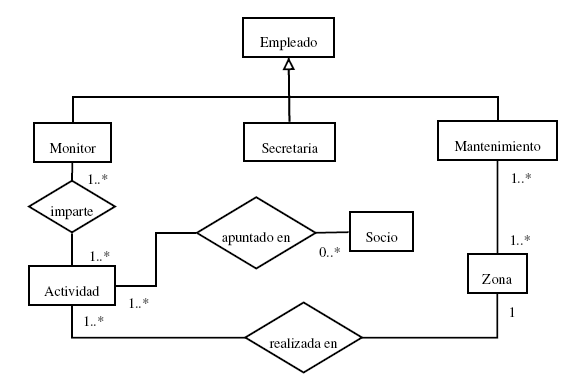
\includegraphics[scale=0.8]{ERe.png}
  \end{center}
  \caption{Diagrama ERe de ejemplo}
\end{figure}


\section{Código fuente}

En \LaTeX tenemos varias maneras de colocar nuestro código fuente, pero
vamos a mostrar dos básicas.

\subsection{Entorno \texttt{Verbatim}}

Este entorno, nos permite incluir dentro de él \negrita{cualquier}
código, y nos respetará espacios, saltos de lineas, tabuladores... es
decir, el compilador de \LaTeX no procesará ese entorno y lo dejará
tal cual está. Veamos un ejemplo con el clásico programa
\programa{Hola mundo} en \texttt{C++}:

\begin{verbatim}
/*Clásico programa en su versión C++*/

#include <iostream>

using namespace std;

int main()
{
  cout << "¡Hola, mundo!" << endl;
  return 0; //No hace falta, pero en fin
}
\end{verbatim}

Vemos, que queda un poco ``soso'': no remarca palabras del lenguaje,
le da igual lo que es comentario y lo que es texto, y claro, a la hora
de tener un código relativamente amplio, pues es incomodo verlo tan
plano. Hay alternativas como \texttt{fncyverbatim}, en la cual podemos
formatearlo algo, añadiendo números de lineas, remarcando palabras del
lenguaje y más opciones, pero quizás la siguiente opción sea más
completa:

\subsection{Entorno \texttt{listing}}

Si vemos en el fichero \comando{comandos.sty}, podemos ver varios
estilos definidos para este entorno. ¿En qué consiste? Pues realmente
este entorno, sabiendo de que lenguaje le estamos pasando el código
(admitiendo gran variedad como C, C++, Java, \TeX, SQL, ADA, Python y
muchísimos más), y ciertas opciones, podemos formatear el código.\\

Este entorno podemos llamarlo de dos formas distintas, la primera es
utilizando un entorno propiamente dicho, con sus
$\backslash$\texttt{begin} y $\backslash$\texttt{end} dentro del cual
copiamos el código, y otra usando el comando
$\backslash$\texttt{lstinputlisting}, pasándole de parámetro el propio
fichero. Veamos de las dos formas:

\begin{lstlisting}[style=C++]
/*Clasico programa en su version C++*/

#include <iostream>

using namespace std;

int main()
{
  cout << "Hola, mundo!" << endl;
  return 0; //No hace falta, pero en fin
}  
\end{lstlisting}

O de la segunda forma:

\lstinputlisting[style=C++]{hola_mundo.cpp}

Notar que uso el estilo \texttt{C++} porque ya lo tengo definido en el
fichero mencionado anteriormente, pero se pueden añadir varios más,
modificando los colores, si queremos o no número de lineas, o por
ejemplo comandos de consola:

\begin{lstlisting}[style=consola]
  g++ hola_mundo.cpp -o hola_mundo
\end{lstlisting}

Desde luego, es bastante más agradable para la vista, lo cual facilita
si lectura. Sin embargo, si usamos esta última opción probablemente
tengamos problemas con los caracteres españoles, acentos y demás,
debido a las diferencias de codificación entre ISO Latin-1 y UTF8. Hay
que tener cuidado en tenerlo todo en UTF8 para que el compilador
``entienda'' los caracteres.

\chapter{Análisis de requisitos}
% -*-cap2.tex-*-
% Este fichero es parte de la plantilla LaTeX para
% la realización de Proyectos Final de Carrera, protejido
% bajo los términos de la licencia GFDL.
% Para más información, la licencia completa viene incluida en el
% fichero fdl-1.3.tex

% Copyright (C) 2009 Pablo Recio Quijano 

En este capítulo se describen todos los aspectos relacionados con el análisis de requisitos del sistema: catálogo de requisitos, modelo conceptual, así como la solución propuesta.

\section{Especificación de requisitos del sistema}

En esta sección se detallan todos los tipos de requisitos necesarios para satisfacer los objetivos y características descritas en las secciones anteriores del presente documento.\\

\subsection{Requisitos de interfaces externas}

En este apartado se describirán los requisitos de conexión del software y el hardware, así como la interfaz de usuario.\\

Sobre la conexión entre el software y el hardware se encarga el SDK de Android, por lo que al ser un sistema preestablecido, no será necesario realizar el diseño ni el análisis; tan solo haremos uso de él.\\

A continuación, pasamos a definir la interfaz de la aplicación. Todas las ventanas de la aplicación se adaptarán a la resolución nativa del dispositivo en que se ejecute.\\

El usuario utilizará la pantalla táctil para interactuar con la interfaz. Por defecto, bastará con una pulsación típica para activar el evento correspondiente. En caso contrario, se mencionará explícitamente.\\

Las diferentes pantallas que modelarán la aplicación serán:

\begin{itemize}
\item \textbf{Pantalla principal}: Es la pantalla inicial, y tiene como función ofrecer al usuario el listado de personas mayores que ha registrado en la aplicación, así como la posibilidad de acceder a las siguientes pantallas:
\begin{itemize}
\item Pantalla de registro de personas
\item Pantalla de selección de persona para comenzar o continuar con una sesión
\item Pantalla de detalle de persona
\end{itemize}
\item \textbf{Registro de personas}: Permite al usuario registrar a personas en el sistema. La información introducida será validada y almacenada en la base de datos. Además dará la posibilidad de tomar una foto con la cámara o bien seleccionar una imagen de la galería para asignarla al usuario. Una vez seleccionada la imagen, debe mostrar al usuario una pantalla de edición que permita recortar la imagen con la proporción de aspecto usada por la aplicación.
\item \textbf{Selección de persona para comenzar o continuar con una sesión}: Permite al usuario seleccionar una persona de entre todas las registradas en la aplicación. Una vez seleccionada, llevará a la pantalla de selección de test.
\item \textbf{Detalle de persona}: Muestra al usuario los datos de la persona que se está consultando, así como un listado de las sesiones realizadas por el mismo, encabezado por aquella sesión que esté en progreso en caso de existir. Además da la posibilidad al usuario de eliminar a la persona, así como de acceder a la pantalla de estadísticas de cualquier sesión ya realizada o a la pantalla de selección de test para aquella sesión que esté en progreso.
\item \textbf{Selección de test}: Muestra al usuario el listado de tests que la persona seleccionada debe realizar. Se indicarán aquellos tests que ya se hayan completado y el resultado obtenido, diferenciándolos de aquellos que estén pendientes de hacer. Además, al lado de cada test aparecerá un botón de información, que de ser pulsado mostrará una pantalla de información sobre el test a realizar.
\item \textbf{Información de test}: Muestra al usuario una breve explicación que indica en qué consiste el ejercicio que se debe realizar para completar el test, así como instrucciones para su correcta realización con el dispositivo móvil en caso de ser necesario. A esta pantalla se accederá desde la pantalla de selección de test.
\item \textbf{Estadísticas de sesión}: Muestra al usuario los resultados obtenidos en los diferentes tests de una sesión ya realizada por una persona, así como estadísticas sobre la misma. A esta pantalla se accederá desde la pantalla de detalle de persona.
\item \textbf{Resultados}: Esta pantalla es la que se muestra al usuario inmediatamente después de que la persona que esté realizando una sesión haya terminado el último test de la misma que tuviese pendiente. En la pantalla se indicarán los resultados obtenidos en la sesión para cada uno de los tests realizados.
\item \textbf{Fuerza de piernas}: En esta pantalla se lleva a cabo la realización del test Fuerza de piernas (F\_Pna). Permite al usuario especificar el tiempo (en segundos) que durará la prueba y unos botones que servirán para iniciar/parar/resetear la prueba. Durante la realización del ejercicio irá mostrando en pantalla el número de repeticiones realizadas, así como una cuenta atrás con el tiempo restante. Una vez haya finalizado el tiempo, mostrará un botón que permitirá almacenar el resultado obtenido para la persona que ha realizado el ejercicio. A esta pantalla se accederá desde la pantalla de selección de test.
\item \textbf{Fuerza de brazos}: En esta pantalla se lleva a cabo la realización del test Fuerza de brazos (F\_Br). Permite al usuario especificar el tiempo (en segundos) que durará la prueba y unos botones que servirán para iniciar/parar/resetear la prueba. Durante la realización del ejercicio irá mostrando en pantalla el número de repeticiones realizadas, así como una cuenta atrás con el tiempo restante. Una vez haya finalizado el tiempo, mostrará un botón que permitirá almacenar el resultado obtenido para la persona que ha realizado el ejercicio. A esta pantalla se accederá desde la pantalla de selección de test.
\item \textbf{Resistencia aeróbica}: En esta pantalla se lleva a cabo la realización del test Resistencia aeróbica (Resist). Permite al usuario especificar el tiempo (en segundos) que durará la prueba y unos botones que servirán para iniciar/parar/resetear la prueba. Durante la realización del ejercicio irá mostrando en pantalla el número de repeticiones realizadas, así como una cuenta atrás con el tiempo restante. Una vez haya finalizado el tiempo, mostrará un botón que permitirá almacenar el resultado obtenido para la persona que ha realizado el ejercicio. A esta pantalla se accederá desde la pantalla de selección de test.
\item \textbf{Flexibilidad de piernas}: En esta pantalla se debe introducir la distancia en centímetros obtenida tras la realización del text Flexibilidad de piernas (Flex\_Pna), y debe contener un botón que tras pulsarse almacenará en el sistema el valor para la persona que esté realizando la sesión. A esta pantalla se accederá desde la pantalla de selección de test.
\item \textbf{Flexibilidad de brazos}: En esta pantalla se debe introducir la distancia en centímetros obtenida tras la realización del text Flexibilidad de brazos (Flex\_Br), y debe contener un botón que tras pulsarse almacenará en el sistema el valor para la persona que esté realizando la sesión. A esta pantalla se accederá desde la pantalla de selección de test.
\item \textbf{Agilidad}: Esta pantalla mostrará al usuario un cronómetro con los controles correspondientes para iniciarlo, pausarlo y resetearlo. Además mostrará un botón que tras pulsarse almacenará en el sistema el tiempo obtenido (en segundos) para la persona que esté realizando el ejercicio. A esta pantalla se accederá desde la pantalla de selección de test.
\end{itemize}

\subsection{Requisitos funcionales}

Los requisitos funcionales se han agrupado en diferentes subsistemas, cada uno de éstos contienen los requisitos establecidos que permitirán cumplir los objetivos y características descritas en las secciones anteriores y que se detallarán más adelante.\\

Para describir los distintos comportamientos que tendrá el sistema, usaremos el lenguaje de modelado de sistemas UML, que representa los requisitos funcionales del sistema, centrado en qué hace y no cómo lo hace.

\subsubsection{4.1.2.1. Diagramas de casos de uso}

Para no sobrecargar el diagrama de casos de uso, se ha optado por dividirlos de la siguiente forma:
\begin{itemize}
\item Un diagrama de casos de uso que mostrará de forma global las funcionalidades de la aplicación.
\item Un diagrama de casos de uso para cada uno de los diferentes tests que componen la Senior Fitness Test.
\end{itemize}

A continuación se muestran los diagramas de casos de uso comentados:

\figura{casosdeusoUML.png}{scale=0.6}{Diagrama UML: Casos de uso de la aplicación}{casosdeuso_uml}{H}

\figura{casosdeusoUMLfuerza_resistencia.png}{scale=0.6}{Diagrama UML: Casos de uso test fuerza de piernas}{casosdeuso_fuerza_piernas}{H}

\figura{casosdeusoUMLfuerza_resistencia.png}{scale=0.6}{Diagrama UML: Casos de uso test fuerza de brazos}{casosdeuso_fuerza_brazos}{H}

\figura{casosdeusoUMLfuerza_resistencia.png}{scale=0.6}{Diagrama UML: Casos de uso test resistencia aeróbica}{casosdeuso_resistencia_aerobica}{H}

\figura{casosdeusoUMLagilidad.png}{scale=0.6}{Diagrama UML: Casos de uso test agilidad}{casosdeuso_agilidad}{H}

\figura{casosdeusoUMLflexibilidad.png}{scale=0.6}{Diagrama UML: Casos de uso test flexibilidad de piernas}{casosdeuso_agilidad}{H}

\figura{casosdeusoUMLflexibilidad.png}{scale=0.6}{Diagrama UML: Casos de uso test flexibilidad de brazos}{casosdeuso_agilidad}{H}

\subsubsection{4.1.2.2. Descripción de casos de uso}

A continuación se detallarán los casos de uso empleados en cada uno de los subsistemas.

\subsubsection{4.1.2.2.1. Subsistema de registro de personas mayores}

\begin{table}[H]
\label{CU01}
\begin{center}
\begin{tabular}{| l | p{10cm} |}
\hline
CU01 & Registrar persona.\\
\hline
Descripción & La persona se registra en el sistema indicando sus datos.\\
\hline
Precondición & El usuario debe encontrarse en la pantalla de registro de personas.\\
\hline
Secuencia normal & 1. El usuario pulsa sobre el botón de registro de persona desde la pantalla principal.
\newline 2. Se muestra al usuario la pantalla de registro de persona.
\newline 3. El usuario hace o selecciona una foto de la persona e introduce el DNI, su nombre, apellidos, fecha de nacimiento y género y pulsa sobre Guardar.
\newline 4. El sistema registra la persona y redirige a la pantalla principal de la aplicación.\\
\hline
Secuencia alternativa & 4a. Se ha dejado uno o varios campos vacíos. Vuelve al paso 3.
\newline 4b. Se ha introducido un DNI de persona existente. Vuelve al paso 3.\\
\hline
Postcondición & Se registra a la persona en el sistema exitosamente y redirige a la pantalla principal de la aplicación.\\
\hline
Importancia & Vital.\\
\hline
\end{tabular}
\end{center}
\caption{CU01}
\end{table} 

\subsubsection{4.1.2.2.2. Subsistema de gestión de personas mayores}

\begin{table}[H]
\label{CU02}
\begin{center}
\begin{tabular}{| l | p{10cm} |}
\hline
CU02 & Ver detalle de persona.\\
\hline
Descripción & El usuario visualiza los datos y sesiones realizadas por la persona seleccionada.\\
\hline
Precondición & Debe existir al menos una persona registrada en la aplicación y el usuario debe haber pulsado sobre una persona del listado de personas registradas de la pantalla principal.\\
\hline
Secuencia normal & 1. El usuario pulsa sobre una de las personas listadas en la pantalla principal.
\newline 2. Se muestra al usuario la pantalla de detalle de persona, donde se encuentran los datos de la misma y un listado de las sesiones realizadas.\\
\hline
Secuencia alternativa & No hay.\\
\hline
Postcondición & Se visualizan los datos de la persona seleccionada y se muestra el listado de sesiones realizadas y la sesión que actualmente tenga en progreso la persona, en caso de que tuviese alguna.\\
\hline
Importancia & Vital.\\
\hline
\end{tabular}
\end{center}
\caption{CU02}
\end{table} 

\begin{table}[H]
\label{CU03}
\begin{center}
\begin{tabular}{| l | p{10cm} |}
\hline
CU03 & Eliminar persona.\\
\hline
Descripción & El usuario elimina la persona seleccionada del sistema, así como todos los datos y resultados asociados a la misma.\\
\hline
Precondición & El usuario debe estar en la pantalla de detalle de usuario, por lo que debe existir al menos una persona registrada en la aplicación y el usuario debe haber pulsado sobre una persona del listado de personas registradas de la pantalla principal.\\
\hline
Secuencia normal & 1. El usuario pulsa sobre una de las personas listadas en la pantalla principal.
\newline 2. Se muestra al usuario la pantalla de detalle de persona, donde se encuentran los datos de la misma y un listado de las sesiones realizadas.
\newline 3. El usuario pulsa sobre el icono de la papelera, situado en la esquina superior izquierda.
\newline 4. Se muestra al usuario un popup de confirmación, donde el usuario puede confirmar o cancelar la acción.
\newline 5. El usuario confirma la acción y el sistema elimina la persona seleccionada y retorna al usuario a la pantalla principal de la aplicación.\\
\hline
Secuencia alternativa & 5a. El usuario cancela la acción. Vuelve al paso 2.\\
\hline
Postcondición & Se elimina la persona seleccionada del sistema exitosamente, así como los datos y resultados asociados a la misma.\\
\hline
Importancia & Vital.\\
\hline
\end{tabular}
\end{center}
\caption{CU03}
\end{table} 

\subsubsection{4.1.2.2.3. Subsistema de gestión de sesiones}

\begin{table}[H]
\label{CU04}
\begin{center}
\begin{tabular}{| l | p{10cm} |}
\hline
CU04 & Comenzar sesión.\\
\hline
Descripción & El usuario pulsa sobre el botón de la pesa situado en la esquina superior derecha de la pantalla principal y la aplicación muestra el listado de personas registradas en el sistema para que el usuario seleccione la persona que comenzará la sesión.\\
\hline
Precondición & Debe existir al menos una persona registrada en la aplicación y el usuario debe haber pulsado sobre el botón de la pesa situado en la esquina superior derecha de la pantalla principal.\\
\hline
Secuencia normal & 1. El usuario pulsa sobre el icono de la pesa situado en la esquina superior derecha de la pantalla principal.
\newline 2. Se muestra la pantalla el listado de personas registradas en la aplicación.\\
\hline
Secuencia alternativa & 2a. Si no hay ninguna persona registrada en la aplicación, se muestra un mensaje indicando que debe existir al menos una persona registrada en el sistema.\\
\hline
Postcondición & Se muestra el listado de personas registradas en la aplicación para que el usuario seleccione la persona que comenzará la sesión.\\
\hline
Importancia & Vital.\\
\hline
\end{tabular}
\end{center}
\caption{CU04}
\end{table}

\begin{table}[H]
\label{CU05}
\begin{center}
\begin{tabular}{| l | p{10cm} |}
\hline
CU05 & Seleccionar persona.\\
\hline
Descripción & El usuario pulsa sobre uno de los usuarios listados y, en caso de que el usuario no tenga ningúna sesión en progreso, se creará la sesión en el sistema para el usuario seleccionado. Por último se mostrará la pantalla de selección de test.\\
\hline
Precondición & El usuario se debe encontrar en la pantalla de selección de usuario y debe existir al menos una persona registrada en la aplicación.\\
\hline
Secuencia normal & 1. El usuario selecciona una de las personas listadas.
\newline 2. Se crea la sesión en el sistema para la persona seleccionada en caso de que el usuario no tuviese ninguna sesión en progreso.
\newline 3. Se muestra la pantalla de selección de test.\\
\hline
Secuencia alternativa & 2a. La persona seleccionada ya tiene una sesión creada y en progreso. Salta al punto 3, mostrándose los resultados obtenidos en aquellos tests que ya hayan sido completados para la sesión que tiene en progreso.\\
\hline
Postcondición & Se crea la sesión en el sistema satisfactoriamente para la persona seleccionada en caso de que no tuviese ninguna sesión en progreso y se muestra al usuario la pantalla de selección de test.\\
\hline
Importancia & Vital.\\
\hline
\end{tabular}
\end{center}
\caption{CU05}
\end{table}

\begin{table}[H]
\label{CU06}
\begin{center}
\begin{tabular}{| l | p{10cm} |}
\hline
CU06 & Seleccionar test.\\
\hline
Descripción & El usuario pulsa sobre uno de los test listados que no estén ya completados y se mostrará la pantalla de realización del test correspondiente.\\
\hline
Precondición & El usuario debe encontrarse en la pantalla de selección de test y la persona seleccionada debe tener una sesión creada y no completada.\\
\hline
Secuencia normal & 1. El usuario selecciona uno de los tests que no estén ya completados.
\newline 2. Se muestra la pantalla de realización del test correspondiente.\\
\hline
Secuencia alternativa & 1a. El usuario selecciona un test que ya estaba completado. Se muestra un mensaje en pantalla indicando que el test ya ha sido realizado y el usuario permanece en la pantalla de selección de test.\\
\hline
Postcondición & Se accede satisfactoriamente a la pantalla de realización del test.\\
\hline
Importancia & Vital.\\
\hline
\end{tabular}
\end{center}
\caption{CU06}
\end{table}

\begin{table}[H]
\label{CU07}
\begin{center}
\begin{tabular}{| l | p{10cm} |}
\hline
CU07 & Ver información de test.\\
\hline
Descripción & El usuario pulsa sobre el icono de información situado a la derecha de cada test en la pantalla de selección de test. El sistema entonces muestra una pantalla con explicaciones sobre cómo realizar el test para el que se está consultando la información.\\
\hline
Precondición & El usuario debe encontrarse en la pantalla de selección de test y la persona seleccionada debe tener una sesión creada y no completada.\\
\hline
Secuencia normal & 1. El usuario pulsa sobre el botón de información que aparece a la derecha de los tests no completados en la pantalla de selección de test.
\newline 2. Se muestra la pantalla de información del test, con las explicaciones pertinentes sobre como realizar el ejercicio.\\
\hline
Secuencia alternativa & No hay.\\
\hline
Postcondición & Se accede satisfactoriamente a la pantalla de información del test.\\
\hline
Importancia & Vital.\\
\hline
\end{tabular}
\end{center}
\caption{CU07}
\end{table}

\begin{table}[H]
\label{CU08}
\begin{center}
\begin{tabular}{| l | p{10cm} |}
\hline
CU08 & Reanudar sesión\\
\hline
Descripción & El usuario pulsa sobre la sesión en progreso que aparece listada en la pantalla de detalle de persona, mostrándose la pantalla de selección de test.\\
\hline
Precondición & El usuario debe encontrarse en la pantalla de detalle de usuario y la persona seleccionada debe tener una sesión creada y no completada.\\
\hline
Secuencia normal & 1. El usuario pulsa sobre la sesión en progreso listada para el usuario del que estamos consultando el detalle.
\newline 2. Se muestra la pantalla de selección de test, diferenciando aquellos que ya estén completados de los pendientes y mostrando los resultados para los que ya están realizados por el usuario para esa sesión.\\
\hline
Secuencia alternativa & No hay.\\
\hline
Postcondición & Se accede satisfactoriamente a la pantalla de selección de test y se muestran los resultados de aquellos que ya estuviesen completados para la sesión, en caso de que los hubiese.\\
\hline
Importancia & Vital.\\
\hline
\end{tabular}
\end{center}
\caption{CU08}
\end{table}

\subsubsection{4.1.2.2.4. Subsistema de resultados y cálculos de estadísticas}

\begin{table}[H]
\label{CU09}
\begin{center}
\begin{tabular}{| l | p{10cm} |}
\hline
CU09 & Ver estadísticas de sesión\\
\hline
Descripción & El usuario pulsa sobre cualquier sesión ya completada de las que aparecen listadas en la pantalla de detalle de persona, mostrándose la pantalla de estadísticas de la sesión.\\
\hline
Precondición & El usuario debe encontrarse en la pantalla de detalle de usuario y la persona seleccionada debe tener al menos una sesión ya completada.\\
\hline
Secuencia normal & 1. El usuario pulsa sobre cualquiera de las sesiones listadas como completadas para el usuario del que estamos consultando el detalle.
\newline 2. Se muestra la pantalla de estadísticas de la sesión completada seleccionada en el paso anterior.\\
\hline
Secuencia alternativa & No hay.\\
\hline
Postcondición & Se accede satisfactoriamente a la pantalla de estadísticas de la sesión completada seleccionada en la pantalla de detalle de usuario.\\
\hline
Importancia & Vital.\\
\hline
\end{tabular}
\end{center}
\caption{CU09}
\end{table}

\begin{table}[H]
\label{CU10}
\begin{center}
\begin{tabular}{| l | p{10cm} |}
\hline
CU10 & Mostrar resultados\\
\hline
Descripción & Cuando el usuario realiza el último test que quede por completar de la sesión, se mostrará al usuario la pantalla de resultados, que mostrará los resultados obtenidos en cada uno de los tests durante la sesión que se acaba de completar.\\
\hline
Precondición & El usuario debe haber completado todos los tests de la sesión que en ese momento tuviese en progreso.\\
\hline
Secuencia normal & 1. El usuario completa el último test que tuviese pendiente de la sesión que tuviese en progreso en el momento de la realización del test indicado.
\newline 2. Una vez obtenido el resultado del último test, se muestra la pantalla de resultados de todos los tests completados para la sesión que recién se ha acabado de completar.\\
\hline
Secuencia alternativa & 1a. El test que se ha completado no era el último y había algún test más pendiente para la sesión actual. Se vuelve a la pantalla de selección de test.\\
\hline
Postcondición & Se muestra satisfactoriamente la pantalla de resultados de la sesión, mostrándose los valores obtenidos para cada uno de los tests que se han completado.\\
\hline
Importancia & Vital.\\
\hline
\end{tabular}
\end{center}
\caption{CU10}
\end{table}

\subsubsection{4.1.2.2.5. Tests de valoración de la condición física}

\subsection{Requisitos no funcionales}

En este apartado se detallarán los requisitos no funcionales del sistema.

\begin{table}[H]
\label{RNF01}
\begin{center}
\begin{tabular}{| l | p{10cm} |}
\hline
RNF01 & Usabilidad.\\
\hline
Descripción & El sistema debe ser usable y disponer de una interfaz intuitiva, adaptable y fácil de manejar para un usuario de nivel básico.\\
\hline
Importancia & Vital.\\
\hline
\end{tabular}
\end{center}
\caption{RNF01}
\end{table} 

\begin{table}[H]
\label{RNF02}
\begin{center}
\begin{tabular}{| l | p{10cm} |}
\hline
RNF02 & Portabilidad.\\
\hline
Descripción & Debe ser posible usar la aplicación en diferentes dispositivos móviles Android, independientemente del tamaño de la pantalla de los mismos, gracias al diseño adaptable empleado en las interfaces de usuario.\\
\hline
Importancia & Vital.\\
\hline
\end{tabular}
\end{center}
\caption{RNF02}
\end{table}

\begin{table}[H]
\label{RNF03}
\begin{center}
\begin{tabular}{| l | p{10cm} |}
\hline
RNF03 & Escabilidad.\\
\hline
Descripción & El sistema debe responder de manera óptima y eficiente a futuras mejoras en el desarrollo de la aplicación, sin que éstas comprometan el estado de la misma. El código debe ser mantenible y fácilmente ampliable para futuras versiones.\\
\hline
Importancia & Vital.\\
\hline
\end{tabular}
\end{center}
\caption{RNF03}
\end{table}

\begin{table}[H]
\label{RNF04}
\begin{center}
\begin{tabular}{| l | p{10cm} |}
\hline
RNF04 & Seguridad\\
\hline
Descripción & Cuando la aplicación necesite hacer uso de algunas características del dispositivo móvil que puedan comprometer la privacidad/seguridad de los datos del usuario, como puede ser la cámara o el acceso de lectura/escritura a los archivos de la memoria del dispositivo, siempre solicitará permiso al usuario antes de hacer uso de las mismas. En caso de que no se conceda el permiso, la aplicación seguirá siendo funcional aunque no se pueda hacer uso de las características para las que no se ha concedido el permiso.\\
\hline
Importancia & Vital.\\
\hline
\end{tabular}
\end{center}
\caption{RNF04}
\end{table} 

\begin{table}[H]
\label{RNF05}
\begin{center}
\begin{tabular}{| l | p{10cm} |}
\hline
RNF05 & Rendimiento\\
\hline
Descripción & El rendimiento de la aplicación de ser tal que permita un desempeño agradable y suave durante el uso de la misma. Los tiempos de respuesta al insertar/recuperar información en la base de datos serán cortos y deberá minimizarse la utilización de recursos cuando sea posible para ahorrar batería.\\
\hline
Importancia & Vital.\\
\hline
\end{tabular}
\end{center}
\caption{RNF05}
\end{table}

\begin{table}[H]
\label{RNF06}
\begin{center}
\begin{tabular}{| l | p{10cm} |}
\hline
RNF06 & Diseño\\
\hline
Descripción & Como se ha indicado en el requisito anterior, minimizar la utilización de recursos y el tiempo de respuesta debe primar sobre cualquier factor. Sin embargo, se debe tener en cuenta que los dispositivos móviles Android (Java) pueden perder el contexto de la aplicación que ejecutan, por lo que el contenido debe ser recuperable. Será de valor añadido que el paquete .APK final tenga el menor tamaño posible para abarcar aquellos teléfonos con menos memoria secundaria.\\
\hline
Importancia & Vital.\\
\hline
\end{tabular}
\end{center}
\caption{RNF06}
\end{table}

\subsection{Reglas de negocio}

El sistema en su totalidad está desarrollado para ser software libre bajo licencia GNU GPL. Ello permite que el código sea accesible a cualquier desarrollador que quiera incrementar su funcionalidad y contribuir a la libre creación de contenidos. Así mismo, las herramientas y tecnologías empleadas también son de libre uso.

\subsection{Requisitos de información}

A continuación se detallarán los requisitos de información, que describen cómo gestiona el sistema la información que se va a almacenar, y son los siguientes:

\section{Modelo conceptual de datos}

En esta sección se muestra el diagrama conceptual de datos UML de la aplicación, con el que se visualizarán a modo de primer vistazo las clases que posteriormente se diseñarán e implementarán para cubrir las funcionalidades impuestas en el proyecto.\\

No será hasta el capítulo siguiente cuando se desarrolle todo lo que abarca al diseño del sistema, incluido el diseño de clases UML que se genera a partir del conceptual que se muestra a continuación:

\section{Modelo de comportamiento del sistema}

Este modelo de comportamiento especifica como debe actuar el sistema. El sistema es el que engloba todos los objetos, y el modelo consta de dos partes:

\begin{itemize}
\item Diagramas de secuencias del sistema: Muestran la secuencia de eventos entre el usuario y el sistema.
\item Contrato de las operaciones del sistema: Describen el efecto que producen las operaciones en el sistema.
\end{itemize}

\subsection{Diagramas de secuencia y contrato de las operaciones del sistema}

A continuación se mostrarán los diagramas de secuencia. Para evitar contenidos duplicados, se omitirán las operaciones que ya hayan sido explicadas con anterioridad.
















\chapter{Diseño del sistema}
% -*-cap2.tex-*-
% Este fichero es parte de la plantilla LaTeX para
% la realización de Proyectos Final de Carrera, protejido
% bajo los términos de la licencia GFDL.
% Para más información, la licencia completa viene incluida en el
% fichero fdl-1.3.tex

% Copyright (C) 2009 Pablo Recio Quijano 

En este capítulo se describen todos los aspectos relacionados con el diseño del sistema: arquitectura del sistema, patrones de diseño, diseño físico de datos, así como el diseño de la interfaz de usuario.

\section{Arquitectura física del sistema}

A continuación se presentan los elementos hardware que componen la arquitectura física del sistema. Para definirla, se detallarán los componentes a nivel de hardware requeridos para el correcto funcionamiento de la aplicación.\\

Cuando hablamos de un dispositivo móvil o smartphone, nos referimos a los sucesores de los teléfonos móviles sencillos, que han ido evolucionando hasta ser prácticamente ordenadores que caben en nuestros bolsillos o en nuestra palma de la mano, y que además incluyen las funciones básicas de sus antecesores, como pueden ser las llamadas, envío y recibo de sms, mms, etc.\\

En los últimos años los dispositivos móviles han empezado a cobrar importancia debido a su relación entre la potencia y su reducido tamaño, llegando incluso a ser indispensables en ciertos sectores de la sociedad hoy en día.\\

Junto con la aparición de los smartphones se presentaron a su vez los sistemas operativos que éstos dispositivos llevarían integrados como pueden ser Android o IOS, cada uno con características propias, ofreciendo así un entorno de fácil manejo para el usuario final y un sinfín de aplicaciones desarrolladas tanto por empresas como por particulares.\\

Dado que la presente aplicación ha sido desarrollada en Android, los requisitos a nivel de hardware se reducen a los siguientes:

\begin{itemize}
\item Dispositivos: Dispositivo móvil basado en Android.
\item Requisitos mínimos:
\begin{itemize}
\item La versión de Android instalada en el dispositivo debe ser superior o igual a la versión 4.0.3 (ICE\_CREAM\_SANDWICH\_MR1).
\item El dispositivo móvil debe disponer de Acelerómetro y Giroscopio.
\end{itemize}
\end{itemize}

Es conveniente destacar la necesidad de que el dispositivo móvil disponga de Acelerómetro y Giroscopio, dado que la combinación de estos dos sensores hardware son los que permiten que exista el sensor de Gravedad que, a diferencia de los dos sensores anteriormente citados, se trata de un sensor software.

\section{Arquitectura lógica del sistema}

En la arquitectura lógica del sistema se detallan los componentes a nivel de software empleados a lo largo del proyecto, que abarcan tanto al conjunto de aplicaciones, bibliotecas y librerías como al propio software desarrollado para cumplir con los objetivos y requisitos establecidos.

\subsection{Android}

\subsubsection{Introducción}

Android puede entenderse como una plataforma software cuya misión consiste en abstraer el hardware subyacente. Inicialmente fue desarrollado para dispositivos táctiles con recursos limitados, con el fin de facilitar el desarrollo de aplicaciones para dichos dispositivos.\\

La gran diferencia de Android respecto al resto de sistemas operativos para dispositivos móviles es su núcleo basado en GNU/Linux. Esto hace que Android adquiera algunas de las principales características de Linux, convirtiéndose en un software libre, gratuito y multiplataforma. \\

Inicialmente fue desarrollado por Android IC, pero en 2005 fue comprado por Google, y hasta entonces era un sistema operativo muy poco conocido. En el 2007 se fundó la Opend Handset Alliance, una agrupación de empresas de desarrollo de software, hardware y telecomunicaciones con el propósito de avanzar en los estándares abiertos para el desarrollo de software y hardware para dispositivos móviles, y fue entonces cuando se produjo la presentación de Android por parte de Google, liberando gran parte de su código bajo una licencia Apache.\\

El éxito tras la presentación fue escaso, debido a que el sistema operativo se presentó antes de que se comercializara ningún dispositivo que lo incluyese. En la actualidad es el sistema operativo más utilizado.

\subsubsection{Arquitectura}

La arquitectura del sistema Android puede verse como una arquitectura por capas o niveles, de forma que cada nivel puede utilizar servicios ofrecidos por los niveles anteriores y éste, a su vez, proporciona nuevas funciones a los niveles superiores. En la siguiente imagen podemos ver los niveles que componen la arquitectura:

\figura{arquitectura_android.png}{scale=0.9}{Arquitectura Android}{arquitectura_android}{H}

\begin{itemize}
\item \textbf{Aplicaciones:} Constituye el conjunto de aplicaciones presentes en un dispositivo, ya sean las instaladas por el usuario o por defecto, las nativas y las administradas.
\item \textbf{Framework de aplicaciones:} Plataforma de desarrollo que facilita la reutilización de componentes, permite el acceso a los diversos servicios ofrecidos y al hardware de los dispositivos. Los más importantes son:
\begin{itemize}
\item Activity Manager: Conjunto de APIs encargadas de gestionar el ciclo de vida de las aplicaciones.
\item Window Manager: Gestiona las ventanas de una aplicación mediante la librería Surface Manager.
\item Telephone Manager: Compendio de APIs que gestionan las funciones básicas de los teléfonos (llamadas, mensajería, etc).
\item Content Provider: Proporciona los mecanismos necesarios para la comunicación entre aplicaciones.
\item View System: Ofrece los elementos básicos necesarios para la construcción de interfaces.
\item Location Manager: Posibilita a las aplicaciones el acceso a la ubicación del dispositivo.
\item Notification Manager: Permite a las aplicaciones notificar al usuario información asociada a ciertos eventos que ocurran durante la ejecución de una aplicación.
\item XMPP Service: Colección de APIs para el uso de este protocolo de intercambio basado en XML.
\item Resource Manager: Encargado de gestionar todos los elementos que forman parte de una aplicación y son externos al código.
\item Package Manager: Gestor de todos los paquetes instalados en un dispositivo Android y que permite la instalación de nuevos paquetes.
\end{itemize}
\item \textbf{Bibliotecas:} Hacen referencia al conjunto de librerías presentes en Android y proporcionan la mayoría de las características más representativas de esta plataforma. Las principales librerías que podemos encontrar son las siguientes:
\begin{itemize}
\item Surface Manager: Gestión de la pantalla.
\item SQLite: Motor de bases de datos relacionales. Es el motor de bases de datos usado en la presente aplicación.
\item Media Framework: Reproducción de imágenes, vídeo y audio.
\item WebKit: Navegación web.
\item SGL: Gráficos 2D
\item Open GL/ES: Gráficos 3D.
\item FreeType: Renderizado de fuentes.
\item SSL: Comunicación segura mediante sockets.
\item Libcr: Variante optimizada de C.
\end{itemize}
\item \textbf{Android Runtime:} Al mismo nivel que las librerías encontramos el entorno de ejecución, que está constituido por las librerías Java que forman el núcleo del lenguaje y la máquina virtual Dalvik o ART para las versiones más modernas.
\item \textbf{Núcleo Linux:} Se utiliza como una capa de abstracción para el hardware subyacente y por tanto contiene los drivers y controladores necesarios para el correcto funcionamiento del mismo.
\end{itemize}

\subsubsection{Componentes de una aplicación Android}

Los componentes de una aplicación Android son los elementos esenciales que la componen. Cada uno de ellos supone un punto de entrada mediante el cual el sistema puede acceder a la aplicación, aunque no todos suponen puntos de entrada para el usuario.\\

Cada componente es un bloque básico que desempeña un papel específico en el funcionamiento de nuestra aplicación. Existen cuatro tipos diferentes de componentes, cada uno de ellos con un ciclo de vida y propósito único. Los componentes son los que siguen a continuación:

\begin{itemize}
\item \textbf{Actividades o Activities:} Cada actividad o activity respresenta una pantalla de nuestra aplicación. Las actividades trabajan en conjunto para dar una visión coherente de la aplicación, sin embargo, la vida de cada actividad es independiente del resto. El ciclo de vida que sigue una actividad se muestra en la siguiente imagen:
\figura{ciclo_vida_activity.png}{scale=0.9}{Arquitectura Android: Ciclo de vida de una Activity}{ciclo_vida_activity}{H}
\item \textbf{Servicios o Services:} Son componentes que se ejecutan en segundo plano con el fin de realizar operaciones de larga duración o procesos remotos. Los servicios carecen de interfaz y generalmente son llamados por las activities para realizar tareas costosas sin bloquear la interfaz, es decir, se pueden dejar en ejecución en segundo plano o logarlos a una actividad para interactuar con ella. En la siguiente imagen veremos el ciclo de vida de un servicio. En la izquierda está actuando en segundo plano y en la derecha está ligado a una activity:
\figura{ciclo_vida_servicio.png}{scale=0.9}{Arquitectura Android: Ciclo de vida de un Servicio}{ciclo_vida_servicio}{H}
\item \textbf{Proveedor de contenido o Content provider:} El proveedor de contenido gestiona los datos que maneja una aplicación. Controla el acceso a archivos, bases de datos SQLite, etc. Mediante el proveedor de contenidos las aplicaciones pueden consultar y modificar datos de otras aplicaciones siempre que posean los permisos adecuados. La siguiente imagen ilustra cómo una activity puede consultar datos de otra aplicación:
\figura{content_provider.png}{scale=0.9}{Arquitectura Android: Content Provider}{content_provider}{H}
\item \textbf{Receptor de difusiones o Broadcast receiver:} Es el componente encargado de responder a las difusiones o anuncios del sistema (por ejemplo, un anuncio del sistema que indica que queda poca batería). Carece de interfaz, pero debe crear una barra de estado para notificar al usuario cuando detexta una difusión. Una aplicación debe registrar un broadcast receiver para indicar qué difusiones le interesan.
\figura{broadcast_receiver.png}{scale=0.8}{Arquitectura Android: Broadcast Receiver}{broadcast_receiver}{H}
\end{itemize}

\subsubsection{Recursos de una aplicación Android}

Los recursos de una aplicación corresponden con todos los ficheros, imágenes, cadenas de texto, etc, que nuestra aplicación utiliza. Cuando trabajamos desarrollando aplicaciones para Android, las buenas prácticas nos dicen que este tipo de archivos debe mantenerse independientemente al código de la aplicación.\\

Este hecho, conocido como externalización de recursos, permite adaptar un mismo código a dispositivos con diferentes configuraciones y características físicas de una forma prácticamente automática. En la siguiente imagen podemos comprobar cómo quedaría una pantalla que no ha sido adaptada para diferentes dispositivos (parte superior) y una que sí (parte inferior):

\figura{externalizacion_recursos.png}{scale=0.9}{Arquitectura Android: Externalización de recursos}{externalizacion_recursos}{H}

\subsubsection{Manifest de una aplicación Android}

El archivo Manifest es un archivo XML que contiene información esencial para Android acerca de la aplicación. Todas las aplicaciones Android deben tener un archivo AndroidManifest.xml en su directorio raíz.\\

Entre todas las funciones que realiza el archivo manifest, las más significativas son las siguientes:

\begin{itemize}
\item Da nombre al paquete Java de la aplicación.
\item Describe los componentes y qué proceso los hospeda.
\item Contiene la declaración de permisos.
\item Lista las librería necesarias.
\item Declara el nivel mínimo de la API de Android requerido.
\end{itemize}

\subsection{Git}

Git es el software de control de versiones que se ha elegido para el desarrollo del proyecto. Fue desarrollado por Linus Torvalds (creador del sistema operativo Linux) y a día de hoy se usa en grandes proyectos, por ejemplo el propio núcleo de Linux. Como es costumbre en el desarrollo de éste proyecto, Git es software libre distribuido bajo la licencia GPL, lo que lo hace una alternativa libre de usar.\\

Git permite tener el código generado en la implementación del sistema en un repositorio (GitHub) y poder acceder a él remotamente desde cualquier PC, así como poder restaurar versiones anteriores en caso que la actual deba ser reemplazada.\\

Como para cualquier proyecto informático, el uso de un repositorio como GitHub para el alojamiento de la aplicación que nos ocupa se antojó necesario, no sólo por el simple hecho de tener todo el sistema alojado en la nube y disponible para cualquier persona, sino por la seguridad que transmite tener todo el desarrollo en un lugar desde donde sea posible descargarlo en cualquier PC y desarrollarlo en éste, por lo que pudiera suceder a lo largo del desarrollo del proyecto.

\subsection{SQLite}

La plataforma Android proporciona dos herramientas principales para el almacenamiento y consulta de datos estructurados, que ya hemos nombrado en los puntos anteriores:

\begin{itemize}
\item Bases de Datos SQLite.
\item Content providers.
\end{itemize}

En este punto nos centraremos en la primera opción, que es la que se usará en la aplicación implementada para el presente proyecto, y que abarcará todas las tareas relacionadas con el almacenamiento de los datos propios de nuestra aplicación.\\

SQLite es un sistema gestor de base de datos relacional (RDBMS) basado en el Lenguaje Estructurado de Consultas (SQL), tal y como sugiere su nombre. Lo que hace único a SQLite es que se considera una solución embebida. La mayoría de los sistemas de gestión de bases de datos como Oracle, MySQL y SQL Server son procesos de servidor autónomos que se ejecutan independientemente, mientras que SQLite es en realidad una librería que está enlazada dentro de las aplicaciones.\\

Se trata de un motor de bases de datos muy popular en la actualidad por ofrecer características tan interesantes como su pequeño tamaño, no necesitar servidor, precisar poca configuración, ser transaccional y por supuesto ser de código libre.\\

Android incorpora de serie todas las herramientas necesarias para la creación y gestión de bases de datos SQLite, y entre ellas una completa API para llevar a cabo de manera sencilla todas las tareas necesarias.\\

En Android, la forma típica de crear, actualizar y conectar con una base de datos SQLite será a través de una clase auxiliar llamada SQLiteOpenHelper, o para ser más exactos, de una clase propia que derive de ella y que debemos personalizar para adaptarnos a las necesidades concretas de nuestra aplicación.

\section{Patrones de diseño}

Los patrones de diseño se pueden definir como los esqueletos de las soluciones a problemas comunes en el desarrollo de software. Éstos brindan una solución ya probada y documentada a problemas de desarrollo de software que están sujetos a contextos similares.\\

Para que una solución sea considerada un patrón, debe poseer ciertas características. Una de ellas es que debe haber comprobado su efectividad resolviendo problemas similares en ocasiones anteriores. Otra es que debe ser reutilizable, lo que significa que es aplicable a diferentes problemas de diseño en distintas circunstancias.\\

Los patrones de diseño pretenden:

\begin{itemize}
\item Proporcionar catálogos de elementos reusables en el diseño de sistemas software.
\item Evitar la reiteración en la búsqueda de soluciones a problemas ya conocidos y solucionados anteriormente.
\item Formalizar un vocabulario común entre diseñadores.
\item Estandarizar el modo en que se realiza el diseño.
\item Facilitar el aprendizaje de las nuevas generaciones de diseñadores, condensando conocimientos ya existentes.
\end{itemize}

Asimismo, no pretenden:

\begin{itemize}
\item Imponer ciertas alternativas de diseño frente a otras.
\item Eliminar la creatividad inherente al proceso de diseño.
\end{itemize}

Para el presente proyecto se han usado patrones de diseño pertenecientes a diferentes subconjuntos de patrones de diseño. Éstos son el patrón Singleton, perteneciente al subconjunto de patrones de diseño creacionales, y el patrón Adapter, perteneciente al subconjunto de patrones de diseño estructurales. A continuación se detallarán ambos para dar conocimiento de cómo funcionan y cómo resuelven determinados problemas del sistema que los implementan.

\subsection{Patrones de diseño creacionales}

Corresponden a patrones de diseño de software que solucionan problemas de creación de instancias. Nos ayudan a encapsular y abstraer dicha creación.

\subsubsection{Patrón de diseño singleton}

El patrón singleton o patrón de instancia única es un patrón de diseño diseñado para restringir la creación de objetos pertenecientes a una clase o el valor de un tipo a un único objeto. Su intención consiste en garantizar que una clase sólo tenga una instancia y proporcionar un punto de acceso global a ella.\\

El patrón singleton se implementa creando en la clase un método que crea una instancia del objeto sólo si todavía no existe alguna. Para asegurar que la clase no puede ser instanciada nuevamente se regula el alcance del constructor haciéndo que éste sea privado y que sea a través de un método específico la manera de crear la primera y única instancia que se va a usar a lo largo del desarrollo.\\

En el desarrollo del presente proyecto, el uso de este patrón se usa para la clase que se ocupa de la definición de la base de datos, ya que a lo largo del proceso de ejecución del sistema sólo es necesario crear una única instancia de dicha clase.\\

\subsection{Patrones de diseño estructurales}

Corresponden a patrones de diseño de software que solucionan problemas de composición (agregación) de clases y objetos.

\subsubsection{Patrón de diseño adapter}

El patrón adapter, también conocido como wrapper, es un patrón de diseño que se utiliza para transformar una interfaz en otra, de tal modo que una clase que no pudiera utilizar otra clase cualquiera, haga uso de ella a través de una segunda. Dicho de otro modo, convierte la interfaz de una clase en otra interfaz que el cliente espera.\\

Este patrón de diseño permite a clases con interfaces incompatibles trabajar juntas mediante un adaptador intermedio, que se encargará de realizar la conversión de una interfaz a otra.\\

En el desarrollo de nuestra aplicación, el uso de este patrón se antoja necesario debido a los listados que se manejan en las diferentes pantallas de la aplicación, dado que, una vez que hemos obtenido de la base de datos el listado de usuarios, tests o sesiones, necesitaremos convertir dichas colecciones de objetos específicos en una colección de vistas (objeto View), que será sobre la que finalmente se iterará en la capa de presentación para pintar cada elemento en la layout correspondiente.

\section{Diseño físico de datos}

En este apartado se detalla el diseño físico de datos usado por nuestra aplicación.\\

Para que se cumplan con los objetivos y los requisitos impuestos en el proyecto, es necesario implementar una estructura capaz de almacenar la información, de forma que se pueda llevar un control y hacer un estudio de los datos obtenidos durante la realización de los tests que componen la batería de pruebas Senior Fitness Test.\\

La información almacenada en la base de datos consistirá tanto en las personas que realizarán los tests, como las sesiones que realizan y los resultados obtenidos en cada una de las pruebas completadas en dichas sesiones.

\subsection{Base de datos}

A continuación se detalla a través del diagrama Entidad-Relación cómo se estructura la base de datos SQLite diseñada para albergar la información citada en el punto anterior.

\figura{modeloconceptual_er_detail.png}{scale=0.9}{Diagrama Entidad-Relación de la base de datos}{ciclo_vida_servicio}{H}

Los atributos identificadores de cada tabla son enteros a excepción del identificador de persona, que se corresponde con el DNI de la misma. Las fechas de los campos date y birthdate son de tipo String pero parseadas desde tipo Date con el siguiente formato dd/MM/yyyy.\\

En el diagrama no se han representado como atributos de las entidades las claves foráneas, aunque sí aparecen en el fichero Contract de la aplicación, en el que se definen la base de datos y así mismo las tablas del proyecto.

\section{Diseño de la interfaz de usuario}

En este punto se especificarán los elementos que componen las distintas interfaces de usuario que existen para la aplicación, detallándose el contenido de cada pantalla representada.\\

Será necesario desarrollar una interfaz sencilla y agradable para el usuario de la aplicación. En el diseño de la misma, se intentará en todo momento que el flujo de ejecución sea lo más intuitivo posible.\\

A continuación se listan las pantallas que componen la aplicación:

\begin{itemize}
\item Pantalla principal.
\item Alta de persona.
\item Detalle de persona.
\item Estadísticas de sesión.
\item Selección de persona.
\item Selección de test.
\item Información de test.
\item Fuerza de piernas.
\item Fuerza de brazos.
\item Resistencia aeróbica.
\item Flexibilidad de piernas.
\item Flexibilidad de brazos.
\item Agilidad.
\item Resultados.
\end{itemize}

No se entrará en detalles sobre el objetivo y funcionalidad de cada pantalla dado que ya fueron descritas en el punto 4.1.1. del presente documento.\\

En el siguiente diagrama podemos ver las distintas opciones de navegación dentro de la aplicación:

\figura{diagrama_pantallas.png}{scale=0.5}{Navegación entre pantallas}{diagrama_pantallas}{H}

\subsection{Pantalla principal}

\figura{pantalla_principal.png}{scale=0.3}{Pantalla principal}{pantalla_principal}{H}

\subsection{Alta de persona}

\figura{alta_persona.png}{scale=0.3}{Pantalla de alta de persona}{alta_persona}{H}

\subsection{Detalle de persona}

\figura{detalle_persona.png}{scale=0.3}{Pantalla de detalle de persona}{detalle_persona}{H}

\subsection{Estadísticas de sesión}

\figura{estadisticas_sesion.png}{scale=0.3}{Pantalla de estadísticas de sesión}{estadisticas_sesion}{H}

\subsection{Selección de persona}

\figura{seleccion_persona.png}{scale=0.3}{Pantalla de selección de persona}{seleccion_persona}{H}

\subsection{Selección de test}

\figura{seleccion_test.png}{scale=0.3}{Pantalla de selección de test}{seleccion_test}{H}

\subsection{Información de test}

\figura{informacion_test.png}{scale=0.3}{Pantalla de información de test}{informacion_test}{H}

\subsection{Fuerza de piernas}

\figura{pantalla_fuerza_piernas.png}{scale=0.3}{Pantalla de test de fuerza de piernas}{pantalla_fuerza_piernas}{H}

\subsection{Fuerza de brazos}

\figura{pantalla_fuerza_brazos.png}{scale=0.3}{Pantalla de test de fuerza de brazos}{pantalla_fuerza_brazos}{H}

\subsection{Resistencia Aeróbica}

\figura{pantalla_resistencia_aerobica.png}{scale=0.3}{Pantalla de test de resistencia aeróbica}{pantalla_resistencia_aerobica}{H}

\subsection{Flexibilidad de piernas}

\figura{pantalla_flexibilidad_piernas.png}{scale=0.3}{Pantalla de test de flexibilidad de piernas}{pantalla_flexibilidad_piernas}{H}

\subsection{Flexibilidad de brazos}

\figura{pantalla_flexibilidad_brazos.png}{scale=0.3}{Pantalla de test de flexibilidad de brazos}{pantalla_flexibilidad_brazos}{H}

\subsection{Agilidad}

\figura{pantalla_agilidad.png}{scale=0.3}{Pantalla de test de agilidad}{pantalla_agilidad}{H}

\subsection{Resultados}

\figura{pantalla_resultados.png}{scale=0.3}{Pantalla de resultados}{pantalla_resultados}{H}

\section{Uso del dispositivo móvil en la realización de ejercicios}

En este punto se definirá cómo debe usarse el dispositivo móvil en aquellos tests de la batería de pruebas Senior Fitness Test en los que podremos usar el dispositivo para que, con ayuda de los diferentes sensores de los que dispone, detecte el movimiento realizado durante los ejercicios, contabilizando de forma autónoma aquellas repeticiones que se realicen de forma satisfactoria.\\

No será hasta el próximo capítulo (Implementación) donde se entre en detalles sobre cómo el dispositivo móvil hace uso de los sensores de movimiento para realizar los cálculos que determinarán si debe contabilizarse una repetición o no.\\

De las seis pruebas que componen la batería Senior Fitness Test, solo tres de ellas harán uso de los sensores de movimiento del dispositivo:

\begin{itemize}
\item Fuerza de piernas.
\item Fuerza de brazos.
\item Resistencia aeróbica.
\end{itemize}

\subsection{Fuerza de piernas (F\_Pna)}

El dispositivo móvil debe ser capaz de contabilizar las repeticiones durante la realización del ejercicio estando éste colocado sobre el muslo de la persona que realiza la prueba. Quedará colocado con la pantalla hacia arriba y de forma que sea legible por la persona cuando ésta se encuentra en el punto de partida del ejercicio, esto es, estando sentada. En la siguiente imagen se ilustra la colocación del dispositivo móvil durante la realización del test:

\figura{dispositivo_movil_piernas.png}{scale=0.6}{Colocación del dispositivo móvil para el test Fuerza de piernas}{dispositivo_movil_piernas}{H}

\subsection{Fuerza de brazos (F\_Br)}

El dispositivo móvil debe ser capaz de contabilizar las repeticiones durante la realización del ejercicio estando éste colocado sobre el antebrazo de la persona que realiza la prueba. Quedará colocado con la pantalla hacia arriba y de forma que sea legible por la persona cuando ésta se encuentra en el punto de partida del ejercicio, esto es, con el brazo extendido. En la siguiente imagen se ilustra la colocación del dispositivo móvil durante la realización del test:

\figura{dispositivo_movil_brazos.png}{scale=0.6}{Colocación del dispositivo móvil para el test Fuerza de brazos}{dispositivo_movil_brazos}{H}

\subsection{Resistencia aeróbica (Resist)}

Al igual que para el test Fuerza de piernas, el dispositivo móvil debe ser capaz de contabilizar las repeticiones durante la realización del ejercicio estando éste colocado sobre el muslo de la persona que realiza la prueba, quedando colocado con la pantalla hacia arriba y de forma que sea legible por la persona cuando ésta se encuentra en el punto de partida del ejercicio (estando de pie en este caso).\\

Cabe destacar que, aunque el dispositivo quede colocado de igual forma que para el ejercicio Fuerza de piernas tal y como ya hemos comentado, diferirá la lectura que el dispositivo móvil tendrá que realizar sobre el movimiento ejecutado, dado que el sentido del movimiento (posición inicial y posición final) no será el mismo para ambos tests.

\section{Diseño de clases UML}

En esta sección se va a mostrar el diseño empleado para el diagrama de clases UML del sistema, que mostrará el diseño de las clases que componen el sistema con sus atributos y métodos necesarios para cumplir con los requisitos y funcionalidades del proyecto expuestas en la etapa de análisis.\\

Dada la naturaleza de las aplicaciones Android, la mayor parte de las clases empleadas en el desarrollo de la aplicación serán activities, y cada una de ellas contendrá la lógica específica de una pantalla de la aplicación.\\

De entre todas las pantallas de la aplicación, hay seis que se corresponden con los tests o pruebas que componen la batería de pruebas Senior Fitness Test (una pantalla para cada test). Al tratarse de pantallas con una finalidad y objetivo similar, hay funcionalidades que comparten entre ellas, por lo que se ha optado por la creación de una activity padre llamada ExerciseActivity de la que extenderán las activities asociadas a cada uno de los tests: fuerza de brazos, fuerza de piernas, resistencia aeróbica, agilidad, flexibilidad de piernas y flexibilidad de brazos, simplificando de esta forma drásticamente el desarrollo de los tests que se vayan implementando sucesivamente tras el primero.\\

\figura{diagrama_clases_uml.png}{scale=0.7}{Diagrama UML con el diseño de clases de la aplicación}{diagrama_clases_uml}{H}

\section{Diseño de componentes}

Para el diseño de componentes se realizarán los diseños de los diagramas de secuencia que muestran el flujo de información existente entre el usuario y los componentes del sistema.

\subsection{Diagramas de secuencia}

Como es sabido de los diagramas de secuencia, éstos representan los flujos de comunicación que se dan para un determinado caso de uso del sistema, por lo que, dados los casos de uso desarrollados en el capítulo de análisis de requisitos para la aplicación que nos ocupa, se procederá a diseñarlos en base a estos diagramas.\\

Cabe destacar que no todos los posibles diagramas de secuencia aparecerán, sino que nos centraremos en aquellos casos de uso de la aplicación que se consideren mas relevantes.

\subsubsection{Diagrama de secuencia de registro de persona}

El diagrama de secuencia para el registro o alta de persona en la aplicación constituye el flujo de comunicación que comienza una vez el usuario pulsa sobre el botón de registro de persona, que lleva a la pantalla donde se encuentra el formulario de datos de registro. En esta página, el usuario rellena los datos y seguidamente pulsa el botón Guardar.\\

Al hacer esto, se ejecutará la función de la activity que nos encontramos encargada de validar los datos introducidos por el usuario. Seguidamente, consultará en la base de datos del sistema si el usuario ya existe en el sistema.\\

Tras la respuesta obtenida, se procede con la inserción de los datos en la base de datos y finalmente se redirige al usuario a la pantalla principal de la aplicación.

\figura{diagrama_secuencia_registro.png}{scale=0.6}{Diagrama de secuencia de registro de persona}{diagrama_secuencia_registro}{H}

\subsubsection{Diagrama de secuencia de comienzo de sesión}

El diagrama de secuencia para el comienzo de sesión en la aplicación constituye el flujo de comunicación que comienza una vez el usuario pulsa sobre el botón correspodiente al icono de las pesas, que se encuentra en la pantalla principal y que lleva a la pantalla de selección de persona.\\

Cuando se accede a la pantalla de selección de persona, el sistema hace una consulta a la base de datos para recuperar el listado de personas que están dadas de alta en la aplicación, y se mostrarán al usuario para que se proceda con la selección de la persona para la cual se creará la sesión en el siguiente paso.\\

\figura{diagrama_secuencia_comienzo_sesion.png}{scale=0.6}{Diagrama de secuencia de registro de comienzo de sesión}{diagrama_secuencia_comienzo_sesion}{H}



\chapter{Implementación del sistema}
% -*-cap2.tex-*-
% Este fichero es parte de la plantilla LaTeX para
% la realización de Proyectos Final de Carrera, protejido
% bajo los términos de la licencia GFDL.
% Para más información, la licencia completa viene incluida en el
% fichero fdl-1.3.tex

% Copyright (C) 2009 Pablo Recio Quijano 

En este capítulo vamos a describir y explicar los detalles de la implementación del sistema software y de la solución propuesta.

\section{Solución propuesta}

Debido a los objetivos y requisitos definidos en las anteriores secciones del documento, ya desde un primer momento se antojaba necesario realizar la implementación de una aplicación móvil, por lo que disponíamos de dos opciones a considerar: hacer una aplicación Android o IOS.\\

Bajo esta disyuntiva, los factores que nos llevaron a tomar la decisión de implementar una aplicación móvil Android fueron los siguientes:

\begin{itemize}
\item Como bien es sabido, la base de Android es Java. Java es uno de los lenguajes más universales y extendidos en el mundo del desarrollo, así que un grandísimo número de desarrolladores lo encontrarán más amigable. Esto, sumado a que desde 2008 me dedico profesionalmente al desarrollo de aplicaciones web con Java, fue un factor determinante a la hora tomar la decisión.
\item Android es un sistema más abierto y "libre" para el desarrollador, permitiéndole tener en una app un control mucho más amplio del terminal que en IOS.
\item La disponibilidad de las herramientas para desarrollar la aplicación también influyó en la decisión. Desarrollar una aplicación IOS requiere hacer uso de un ordenador Mac y de un iPhone para el testeo de la aplicación en el hardware real; herramientas que, teniendo en cuenta que necesitamos hacer uso de los sensores hardware del dispositivo, habría sido necesario adquirir para acometer el desarrollo.
\item Android copa actualmente el 92\% del mercado español \cite{website:cuota}, por lo que por estadística podría hacer uso de la aplicación un público más amplio.
\end{itemize}

Todos estos factores, sumados a la baja curva de aprendizaje necesaria debido principalmente a mi experiencia previa con Java, nos llevaron a seleccionar Android como plataforma de desarrollo.

\section{Entorno de construcción}

Una vez que se ha llegado a la conclusión anterior de implementar la aplicación móvil haciendo uso de Android, se procede a analizar el entorno de construcción que permitirá el desarrollo de todo el sistema.

\subsection{Android Studio}

Para el desarrollo de la aplicación haremos uso del entorno de desarrollo integrado (IDE) Android Studio \cite{website:androidstudio}. Android Studio es el entorno de desarrollo integrado oficial para el desarrollo de aplicaciones para Android y se basa en IntelliJ IDEA.\\

Entre las muchas ventajas que nos ofrece podemos contar con una vista ordenada y modular de los archivos que componen nuestro proyecto. La vista mostrada no se corresponde con la forma original de los archivos en disco, sino que está pensada para optimizar el trabajo.\\

Integrado en nuestro entorno de trabajo, podemos encontrar un sistema para el control de versiones, que incluye soporte para los repositorios más conocidos (Git, Subversion, etc). En nuestro caso se integró con Git, que es el software de control de versiones seleccionado para el presente proyecto, como ya se indicó anteriormente en el documento.\\

La interfaz gráfica está dividida de forma que se muestra una gran cantidad de información de forma eficiente. Además es totalmente personalizable, permitiendo al usuario mostrar y ocultar secciones según se requiera. Android Studio sigue el contexto de trabajo del usuario, mostrando las ventanas con las herramientas que considera oportunas en cada instante.\\

A continuación se muestra un ejemplo de interfaz gráfica:

\figura{androidstudio.png}{scale=0.34}{Interfaz de Android Studio}{androidstudio}{H}

\begin{enumerate}
\item Barra de herramientas: Permite realizar una amplia de gama de acciones: edición, búsqueda, iniciar aplicación, debug, etc. 
\item Barra de navegación: Permite navegar entre los archivos abiertos para facilitar su edición.
\item Ventana de edición: Permite modificar los diferentes archivos.
\item Ventana de herramientas: Proporciona acceso a la gestión del proyecto, control de versiones, consola, etc.
\item Barra de estado: Muestra el estado del proyecto, así como mensajes y avisos.
\end{enumerate}

Para finalizar nuestra visión de Android Studio, finalizaremos hablando de Gradle. Gradle es un sistema abierto que automatiza la compilación del código. Utiliza un grafo dirigido acíclico para determinar en qué orden se pueden ejecutar las tareas. Android Studio incorpora esta tecnología para facilitar la reutilización de código permitiendo generar APKs con distintas funcionalidades partiendo de un mismo proyecto.

\subsection{Android Software Development Kit}

Android SDK o Software Development Kit es un conjunto de herramientas para desarrollar, compilar y depurar aplicaciones para el sistema operativo Android, en definitiva, es una API que además de herramientas para el desarrollo, proporciona soporte técnico, ejemplos y una buena documentación.\\

El SDK incluye un emulador de dispositivos Android, lo que permite probar las aplicaciones de forma rápida y eficiente. Los parámetros de nuestro emulador pueden configurarse de forma que podemos elegir las características que tendrá nuestro dispositivo, como la memoria principal, el tamaño del dispositivo o la versión de Android, lo que permite al programador probar su código en una infinidad de dispositivos sin necesidad de adquirirlos.

\section{Código fuente}

El código fuente desarrollado de la aplicación está alojado en el repositorio GitHub:\\ 

\url{https://github.com/alvarogonzalezalvarez/SeniorFitness}\\

A continuación se muestra una lista con las diferentes clases Java implementadas durante la realización de la aplicación. Junto a cada una de las clases habrá una pequeña descripción sobre la labor que desempeña cada una.

\subsection{Activities}

Una Activity es un componente de la aplicación que contiene una pantalla con la que los usuarios pueden interactuar para realizar una acción. A cada actividad se le asigna una ventana en la que se pinta la interfaz de usuario asociada. A continuación se listan las activities que se han implementado:

\begin{itemize}
\item \textbf{AddUserActivity:} Activity que contiene la lógica de negocio referente a la pantalla de registro/alta de personas. 
\item \textbf{AgilidadActivity:} Activity que contiene la lógica de negocio referente a la pantalla del test Agilidad de la batería de pruebas Senior Fitness Test. Esta actividad extiende a ExerciseActivity.
\item \textbf{ExerciseActivity:} Activity que contiene toda la lógica de negocio común a todos los tests de la batería de pruebas Senior Fitness Test. Provee los métodos y funciones listas para su uso o sobreescritura por cada uno de los tests.
\item \textbf{FlexibilidadBrazosActivity:} Activity que contiene la lógica de negocio referente a la pantalla del test Flexibilidad de brazos de la batería de pruebas Senior Fitness Test. Esta actividad extiende a ExerciseActivity.
\item \textbf{FlexibilidadPiernasActivity:} Activity que contiene la lógica de negocio referente a la pantalla del test Flexibilidad de piernas de la batería de pruebas Senior Fitness Test. Esta actividad extiende a ExerciseActivity.
\item \textbf{FuerzaBrazosActivity:} Activity que contiene la lógica de negocio referente a la pantalla del test Fuerza de brazos de la batería de pruebas Senior Fitness Test. Esta actividad extiende a ExerciseActivity.
\item \textbf{FuerzaPiernasActivity:} Activity que contiene la lógica de negocio referente a la pantalla del test Fuerza de piernas de la batería de pruebas Senior Fitness Test. Esta actividad extiende a ExerciseActivity.
\item \textbf{InfoActivity:} Activity que contiene la lógica de negocio referente a la pantalla de información de los diferentes tests de la batería de pruebas Senior Fitness Test.
\item \textbf{MainActivity:} Activity que contiene la lógica de negocio referente a la pantalla principal de la aplicación. Esta actividad es la que se lanza por defecto cuando se abre la aplicación.
\item \textbf{ResistenciaAerobicaActivity:} Activity que contiene la lógica de negocio referente a la pantalla del test Resistencia aeróbica de la batería de pruebas Senior Fitness Test. Esta actividad extiende a ExerciseActivity.
\item \textbf{ResultsActivity:} Activity que contiene la lógica de negocio referente a la pantalla de resultados mostrada tras finalizar todos los tests de una sesión.
\item \textbf{SelectTestActivity:} Activity que contiene la lógica de negocio referente a la pantalla de selección de los diferentes tests que componen la batería de pruebas Senior Fitness Test.
\item \textbf{StartSessionActivity:} Activity que contiene la lógica de negocio referente a la pantalla de selección de la persona que comenzará la sesión de ejercicios.
\item \textbf{StatsActivity:} Activity que contiene la lógica de negocio referente a la pantalla de estadísticas de una sesión concreta ya completada por la persona para la cual se está visualizando el detalle.
\item \textbf{UserDetailsActivity:} Activity que contiene la lógica de negocio referente a la pantalla de detalle/historial de usuario.
\end{itemize}

\subsection{Listeners}

Los listeners o escuchadores son clases usadas para recibir notificaciones procedentes del SensorManager (clase que nos permite acceder a los sensores del dispositivo). A continuación listamos los listeners que se han implementado.

\begin{itemize}
\item \textbf{ExerciseListener:} Listener que implementa la clase SensorEventListener. Cada vez que hay un evento del sensor usado se invoca el método onSensorChanged, que será el método donde se harán los cálculos necesarios para detectar si el ejercicio se ha realizado de forma satisfactoria. Éste método debe ser implementado por los listeners que extienden de ExerciseListener.
\item \textbf{FuerzaBrazosListener:} Listener encargado de detectar y leer los movimientos realizados durante la realización del test Fuerza de brazos de la batería de pruebas Senior Fitness Test. Este listener extiende a ExerciseListener.
\item \textbf{FuerzaPiernasListener:} Listener encargado de detectar y leer los movimientos realizados durante la realización del test Fuerza de piernas de la batería de pruebas Senior Fitness Test. Este listener extiende a ExerciseListener.
\item \textbf{ResistenciaAerobicaListener:} Listener encargado de detectar y leer los movimientos realizados durante la realización del test Resistencia aeróbica de la batería de pruebas Senior Fitness Test. Este listener extiende a ExerciseListener.
\end{itemize}

\subsection{Base de Datos}

A continuación se listarán las clases encargadas de la definición, gestión y uso de la base de datos:

\begin{itemize}
\item \textbf{SeniorFitnessContract:} Clase java donde se definen las tablas usadas y los nombres y tipos de los campos de cada una de las mismas.
\item \textbf{SeniorFitnessDBHelper:} Clase java que extiende a SQLiteOpenHelper. Se encarga de gestionar la creación y manipulación de la base de datos, así como del versionado de la misma.
\end{itemize}

\subsection{Modelo}

Se listarán a continuación las clases Java que representan el modelo de la aplicación:

\begin{itemize}
\item \textbf{Result:} Clase java que representa los resultados obtenidos, asociado a un test, a una sesión y a una persona.
\item \textbf{Session:} Clase java que representa a las sesiones de tests que realizan las personas dadas de alta en la aplicación.
\item \textbf{Test:} Clase java que representa a los diferentes tests que componen la batería de pruebas Senior Fitness Test.
\item \textbf{User:} Clase java que representa a las personas dadas de alta en la aplicación.
\end{itemize}

\subsection{Adapters}

Un adapter es un objeto que funciona como puente entre un AdapterView y los correspondientes datos para esa vista, proporcionando acceso a los datos del elemento. También es el encargado de construir una vista (View) por cada elemento del conjunto de datos. A continuación listamos los adapters implementados para la aplicación:

\begin{itemize}
\item \textbf{SessionsAdapter:} Adapter utilizado para convertir en una View independiente cada elemento contenido en el listado de sesiones recuperadas para una persona concreta y mostradas en la pantalla de detalle de persona.
\item \textbf{TestsAdapter:} Adapter utilizado para convertir en una View independiente cada elemento contenido en el listado de tests mostrados en la pantalla de selección de test.
\item \textbf{UsersAdapter:} Adapter utilizado para convertir en una View independiente cada elemento contenido en el listado de personas dadas de alta en la aplicación, y que se muestran en la pantalla principal y en la pantalla de selección de persona.
\end{itemize}

\section{Detección de movimiento}





\chapter{Pruebas y validaciones}
% -*-cap2.tex-*-
% Este fichero es parte de la plantilla LaTeX para
% la realización de Proyectos Final de Carrera, protejido
% bajo los términos de la licencia GFDL.
% Para más información, la licencia completa viene incluida en el
% fichero fdl-1.3.tex

% Copyright (C) 2009 Pablo Recio Quijano 

\section{Organización temporal}

En este apartado podemos añadir un diagrama de Gannt, con la
planificación temporal que se realizó del proyecto. Para ello podemos
usar algún programa libre como por ejemplo \programa{Planner}:

\figura{gannt.png}{scale=0.6}{Diagrama de Gannt. Desarrollo del
  proyecto}{gannt}{H}

Observad el código, notareis algo distinto con respecto a las imágenes
del capítulo anterior. En este caso utilizo un comando personalizado
en \comando{comandos.sty}, donde simplifico la creación de una
figura, como en la figura~\ref{gannt}. % Podemos poner o no la ~

\section{Análisis del sistema}

Si el proyecto se refiere a un sistema software, normalmente
procederemos a un análisis y a un diseño del sistema usando notación
UML, para organizar correctamente dicho sistema.\\

\LaTeX{} no trae soporte nativo para hacer este tipo de diagramas, y
aunque se pueden utilizar paquetes que lo hagan. Sin embargo lo más
cómodo es que utilizemos herramientas CASE para ayudarnos a dicha
tarea, como pueden ser \programa{Dia} o \programa{Umbrello}, como
podemos ver en la figura \ref{uml}.

\figura{uml.png}{scale=1}{UML de ejemplo con Umbrello}{uml}{H}

Ya que no es el objetivo de este documento trabajar con dichas
herramientas, aprovecharé este apartado para mostrar algunas
cosas más de las que podemos dotar a nuestro documento \LaTeX{}.\\

Sabemos que tenemos un fichero \texttt{bibliografia.bib}, para que la
herramienta Bib\TeX{}  nos genere las referencias bibliográficas. Sin
embargo a priori no se mostrarán hasta que nos las referenciemos.\\

Teniendo en cuenta que todo esto lo tomamos desde la ``biblia'' de
\LaTeX, podemos hacer una referencia a ella \cite{mitt04}. También hay
que saber que una guia de referencia online muy buena es la página en
\texttt{wikibooks} de \LaTeX{} \cite{website:latex-wikibooks}. 

% TO-DO: Multirow, Multicolumn y Supertabular.

\section{Base de Datos}

Supongamos que en este apartado, queremos incluir un \negrita{diagrama
Entidad-Relación Extendido}, que modele la base de datos que vamos a
utilizar en nuestro proyecto. Una posible herramienta para dibujarla
es \programa{Dia}, una herramienta pra gráficos vectoriales bastante
completa. Una vez hemos hecho el diagrama, podemos importarlo a una
imagen en multitud de formatos, o también podemos a código
\programa{.tex}.\\

¿Qué utilidad tiene esto? Pues basicamente lo podremos modificar para
refinarlo un poco, añadirle fórmulas matemáticas si quisieramos, o
diversas cosas. Además de comprimir bastante en espacio respecto a una
imagen. El diagrama \ref{ERe}, está realizado con Dia importándolo a
\LaTeX{}:

\begin{figure}[H]
  \label{ERe}
  \begin{center}
    % -*-ERe.tex-*-
% Este fichero es parte de la plantilla LaTeX para
% la realización de Proyectos Final de Carrera, protejido
% bajo los términos de la licencia GFDL.
% Para más información, la licencia completa viene incluida en el
% fichero fdl-1.3.tex

% Copyright (C) 2009 Pablo Recio Quijano, Noelia Sales Montes

% necesita \usepackage{tikz}
\ifx\du\undefined
  \newlength{\du}
\fi
\setlength{\du}{15\unitlength}
\begin{tikzpicture}
\pgftransformxscale{1.000000}
\pgftransformyscale{-1.000000}
\definecolor{dialinecolor}{rgb}{0.000000, 0.000000, 0.000000}
\pgfsetstrokecolor{dialinecolor}
\definecolor{dialinecolor}{rgb}{1.000000, 1.000000, 1.000000}
\pgfsetfillcolor{dialinecolor}
\definecolor{dialinecolor}{rgb}{1.000000, 1.000000, 1.000000}
\pgfsetfillcolor{dialinecolor}
\fill (20.800000\du,-5.900000\du)--(20.800000\du,-3.900000\du)--(25.475000\du,-3.900000\du)--(25.475000\du,-5.900000\du)--cycle;
\pgfsetlinewidth{0.100000\du}
\pgfsetdash{}{0pt}
\pgfsetmiterjoin
\definecolor{dialinecolor}{rgb}{0.000000, 0.000000, 0.000000}
\pgfsetstrokecolor{dialinecolor}
\draw (20.800000\du,-5.900000\du)--(20.800000\du,-3.900000\du)--(25.475000\du,-3.900000\du)--(25.475000\du,-5.900000\du)--cycle;
% setfont left to latex
\definecolor{dialinecolor}{rgb}{0.000000, 0.000000, 0.000000}
\pgfsetstrokecolor{dialinecolor}
\node at (23.137500\du,-4.597500\du){Empleado};
\definecolor{dialinecolor}{rgb}{1.000000, 1.000000, 1.000000}
\pgfsetfillcolor{dialinecolor}
\fill (20.840000\du,-0.530000\du)--(20.840000\du,1.470000\du)--(25.542500\du,1.470000\du)--(25.542500\du,-0.530000\du)--cycle;
\pgfsetlinewidth{0.100000\du}
\pgfsetdash{}{0pt}
\pgfsetmiterjoin
\definecolor{dialinecolor}{rgb}{0.000000, 0.000000, 0.000000}
\pgfsetstrokecolor{dialinecolor}
\draw (20.840000\du,-0.530000\du)--(20.840000\du,1.470000\du)--(25.542500\du,1.470000\du)--(25.542500\du,-0.530000\du)--cycle;
% setfont left to latex
\definecolor{dialinecolor}{rgb}{0.000000, 0.000000, 0.000000}
\pgfsetstrokecolor{dialinecolor}
\node at (23.191250\du,0.772500\du){Secretaria};
\definecolor{dialinecolor}{rgb}{1.000000, 1.000000, 1.000000}
\pgfsetfillcolor{dialinecolor}
\fill (10.030000\du,-0.510000\du)--(10.030000\du,1.490000\du)--(13.980000\du,1.490000\du)--(13.980000\du,-0.510000\du)--cycle;
\pgfsetlinewidth{0.100000\du}
\pgfsetdash{}{0pt}
\pgfsetmiterjoin
\definecolor{dialinecolor}{rgb}{0.000000, 0.000000, 0.000000}
\pgfsetstrokecolor{dialinecolor}
\draw (10.030000\du,-0.510000\du)--(10.030000\du,1.490000\du)--(13.980000\du,1.490000\du)--(13.980000\du,-0.510000\du)--cycle;
% setfont left to latex
\definecolor{dialinecolor}{rgb}{0.000000, 0.000000, 0.000000}
\pgfsetstrokecolor{dialinecolor}
\node at (12.005000\du,0.792500\du){Monitor};
\definecolor{dialinecolor}{rgb}{1.000000, 1.000000, 1.000000}
\pgfsetfillcolor{dialinecolor}
\fill (30.822600\du,-0.595000\du)--(30.822600\du,1.405000\du)--(36.982600\du,1.405000\du)--(36.982600\du,-0.595000\du)--cycle;
\pgfsetlinewidth{0.100000\du}
\pgfsetdash{}{0pt}
\pgfsetmiterjoin
\definecolor{dialinecolor}{rgb}{0.000000, 0.000000, 0.000000}
\pgfsetstrokecolor{dialinecolor}
\draw (30.822600\du,-0.595000\du)--(30.822600\du,1.405000\du)--(36.982600\du,1.405000\du)--(36.982600\du,-0.595000\du)--cycle;
% setfont left to latex
\definecolor{dialinecolor}{rgb}{0.000000, 0.000000, 0.000000}
\pgfsetstrokecolor{dialinecolor}
\node at (33.902600\du,0.707500\du){Mantenimiento};
\definecolor{dialinecolor}{rgb}{1.000000, 1.000000, 1.000000}
\pgfsetfillcolor{dialinecolor}
\fill (32.354000\du,6.245200\du)--(32.354000\du,8.245200\du)--(35.431500\du,8.245200\du)--(35.431500\du,6.245200\du)--cycle;
\pgfsetlinewidth{0.100000\du}
\pgfsetdash{}{0pt}
\pgfsetmiterjoin
\definecolor{dialinecolor}{rgb}{0.000000, 0.000000, 0.000000}
\pgfsetstrokecolor{dialinecolor}
\draw (32.354000\du,6.245200\du)--(32.354000\du,8.245200\du)--(35.431500\du,8.245200\du)--(35.431500\du,6.245200\du)--cycle;
% setfont left to latex
\definecolor{dialinecolor}{rgb}{0.000000, 0.000000, 0.000000}
\pgfsetstrokecolor{dialinecolor}
\node at (33.892750\du,7.547700\du){Zona};
\definecolor{dialinecolor}{rgb}{1.000000, 1.000000, 1.000000}
\pgfsetfillcolor{dialinecolor}
\fill (26.282700\du,4.070200\du)--(26.282700\du,6.070200\du)--(29.570200\du,6.070200\du)--(29.570200\du,4.070200\du)--cycle;
\pgfsetlinewidth{0.100000\du}
\pgfsetdash{}{0pt}
\pgfsetmiterjoin
\definecolor{dialinecolor}{rgb}{0.000000, 0.000000, 0.000000}
\pgfsetstrokecolor{dialinecolor}
\draw (26.282700\du,4.070200\du)--(26.282700\du,6.070200\du)--(29.570200\du,6.070200\du)--(29.570200\du,4.070200\du)--cycle;
% setfont left to latex
\definecolor{dialinecolor}{rgb}{0.000000, 0.000000, 0.000000}
\pgfsetstrokecolor{dialinecolor}
\node at (27.926450\du,5.372700\du){Socio};
\pgfsetlinewidth{0.100000\du}
\pgfsetdash{}{0pt}
\pgfsetdash{}{0pt}
\pgfsetbuttcap
{
\definecolor{dialinecolor}{rgb}{0.000000, 0.000000, 0.000000}
\pgfsetfillcolor{dialinecolor}
% was here!!!
\definecolor{dialinecolor}{rgb}{0.000000, 0.000000, 0.000000}
\pgfsetstrokecolor{dialinecolor}
\draw (23.178300\du,-0.580358\du)--(23.137500\du,-3.900000\du);
}
\definecolor{dialinecolor}{rgb}{0.000000, 0.000000, 0.000000}
\pgfsetstrokecolor{dialinecolor}
\draw (23.178300\du,-0.580358\du)--(23.145019\du,-3.288243\du);
\pgfsetmiterjoin
\definecolor{dialinecolor}{rgb}{1.000000, 1.000000, 1.000000}
\pgfsetfillcolor{dialinecolor}
\fill (23.395000\du,-3.291315\du)--(23.138874\du,-3.788205\du)--(22.895038\du,-3.285170\du)--cycle;
\pgfsetlinewidth{0.100000\du}
\pgfsetdash{}{0pt}
\pgfsetmiterjoin
\definecolor{dialinecolor}{rgb}{0.000000, 0.000000, 0.000000}
\pgfsetstrokecolor{dialinecolor}
\draw (23.395000\du,-3.291315\du)--(23.138874\du,-3.788205\du)--(22.895038\du,-3.285170\du)--cycle;
\pgfsetlinewidth{0.100000\du}
\pgfsetdash{}{0pt}
\pgfsetdash{}{0pt}
\pgfsetmiterjoin
\pgfsetbuttcap
{
\definecolor{dialinecolor}{rgb}{0.000000, 0.000000, 0.000000}
\pgfsetfillcolor{dialinecolor}
% was here!!!
{\pgfsetcornersarced{\pgfpoint{0.000000\du}{0.000000\du}}\definecolor{dialinecolor}{rgb}{0.000000, 0.000000, 0.000000}
\pgfsetstrokecolor{dialinecolor}
\draw (33.902600\du,-0.595000\du)--(33.902600\du,-1.839800\du)--(12.005000\du,-1.839800\du)--(12.005000\du,-0.559434\du);
}}
\definecolor{dialinecolor}{rgb}{1.000000, 1.000000, 1.000000}
\pgfsetfillcolor{dialinecolor}
\fill (9.754000\du,3.791450\du)--(11.972750\du,2.460200\du)--(14.191500\du,3.791450\du)--(11.972750\du,5.122700\du)--cycle;
\pgfsetlinewidth{0.100000\du}
\pgfsetdash{}{0pt}
\pgfsetmiterjoin
\definecolor{dialinecolor}{rgb}{0.000000, 0.000000, 0.000000}
\pgfsetstrokecolor{dialinecolor}
\draw (9.754000\du,3.791450\du)--(11.972750\du,2.460200\du)--(14.191500\du,3.791450\du)--(11.972750\du,5.122700\du)--cycle;
% setfont left to latex
\definecolor{dialinecolor}{rgb}{0.000000, 0.000000, 0.000000}
\pgfsetstrokecolor{dialinecolor}
\node[anchor=east] at (9.454000\du,3.491450\du){};
\definecolor{dialinecolor}{rgb}{0.000000, 0.000000, 0.000000}
\pgfsetstrokecolor{dialinecolor}
\node[anchor=west] at (14.491500\du,3.491450\du){};
\definecolor{dialinecolor}{rgb}{0.000000, 0.000000, 0.000000}
\pgfsetstrokecolor{dialinecolor}
\node at (11.972750\du,4.093950\du){imparte};
\pgfsetlinewidth{0.100000\du}
\pgfsetdash{}{0pt}
\pgfsetdash{}{0pt}
\pgfsetbuttcap
{
\definecolor{dialinecolor}{rgb}{0.000000, 0.000000, 0.000000}
\pgfsetfillcolor{dialinecolor}
% was here!!!
\definecolor{dialinecolor}{rgb}{0.000000, 0.000000, 0.000000}
\pgfsetstrokecolor{dialinecolor}
\draw (11.987836\du,1.538593\du)--(11.972750\du,2.460200\du);
}
\pgfsetlinewidth{0.100000\du}
\pgfsetdash{}{0pt}
\pgfsetdash{}{0pt}
\pgfsetbuttcap
{
\definecolor{dialinecolor}{rgb}{0.000000, 0.000000, 0.000000}
\pgfsetfillcolor{dialinecolor}
% was here!!!
\definecolor{dialinecolor}{rgb}{0.000000, 0.000000, 0.000000}
\pgfsetstrokecolor{dialinecolor}
\draw (11.970796\du,5.169007\du)--(11.968437\du,6.832059\du);
}
\definecolor{dialinecolor}{rgb}{1.000000, 1.000000, 1.000000}
\pgfsetfillcolor{dialinecolor}
\fill (18.404000\du,5.147700\du)--(21.466500\du,3.310200\du)--(24.529000\du,5.147700\du)--(21.466500\du,6.985200\du)--cycle;
\pgfsetlinewidth{0.100000\du}
\pgfsetdash{}{0pt}
\pgfsetmiterjoin
\definecolor{dialinecolor}{rgb}{0.000000, 0.000000, 0.000000}
\pgfsetstrokecolor{dialinecolor}
\draw (18.404000\du,5.147700\du)--(21.466500\du,3.310200\du)--(24.529000\du,5.147700\du)--(21.466500\du,6.985200\du)--cycle;
% setfont left to latex
\definecolor{dialinecolor}{rgb}{0.000000, 0.000000, 0.000000}
\pgfsetstrokecolor{dialinecolor}
\node[anchor=east] at (18.104000\du,4.847700\du){};
\definecolor{dialinecolor}{rgb}{0.000000, 0.000000, 0.000000}
\pgfsetstrokecolor{dialinecolor}
\node[anchor=west] at (24.829000\du,4.847700\du){};
\definecolor{dialinecolor}{rgb}{0.000000, 0.000000, 0.000000}
\pgfsetstrokecolor{dialinecolor}
\node at (21.466500\du,5.450200\du){apuntado en};
\pgfsetlinewidth{0.100000\du}
\pgfsetdash{}{0pt}
\pgfsetdash{}{0pt}
\pgfsetbuttcap
{
\definecolor{dialinecolor}{rgb}{0.000000, 0.000000, 0.000000}
\pgfsetfillcolor{dialinecolor}
% was here!!!
\definecolor{dialinecolor}{rgb}{0.000000, 0.000000, 0.000000}
\pgfsetstrokecolor{dialinecolor}
\draw (24.529000\du,5.147700\du)--(26.232300\du,5.108850\du);
}
\pgfsetlinewidth{0.100000\du}
\pgfsetdash{}{0pt}
\pgfsetdash{}{0pt}
\pgfsetmiterjoin
\pgfsetbuttcap
{
\definecolor{dialinecolor}{rgb}{0.000000, 0.000000, 0.000000}
\pgfsetfillcolor{dialinecolor}
% was here!!!
{\pgfsetcornersarced{\pgfpoint{0.000000\du}{0.000000\du}}\definecolor{dialinecolor}{rgb}{0.000000, 0.000000, 0.000000}
\pgfsetstrokecolor{dialinecolor}
\draw (11.966970\du,8.929609\du)--(11.967000\du,10.550000\du)--(33.892750\du,10.550000\du)--(33.892750\du,8.245200\du);
}}
\definecolor{dialinecolor}{rgb}{1.000000, 1.000000, 1.000000}
\pgfsetfillcolor{dialinecolor}
\fill (20.900700\du,10.539700\du)--(23.908200\du,8.735200\du)--(26.915700\du,10.539700\du)--(23.908200\du,12.344200\du)--cycle;
\pgfsetlinewidth{0.100000\du}
\pgfsetdash{}{0pt}
\pgfsetmiterjoin
\definecolor{dialinecolor}{rgb}{0.000000, 0.000000, 0.000000}
\pgfsetstrokecolor{dialinecolor}
\draw (20.900700\du,10.539700\du)--(23.908200\du,8.735200\du)--(26.915700\du,10.539700\du)--(23.908200\du,12.344200\du)--cycle;
% setfont left to latex
\definecolor{dialinecolor}{rgb}{0.000000, 0.000000, 0.000000}
\pgfsetstrokecolor{dialinecolor}
\node[anchor=east] at (20.600700\du,10.239700\du){};
\definecolor{dialinecolor}{rgb}{0.000000, 0.000000, 0.000000}
\pgfsetstrokecolor{dialinecolor}
\node[anchor=west] at (27.215700\du,10.239700\du){};
\definecolor{dialinecolor}{rgb}{0.000000, 0.000000, 0.000000}
\pgfsetstrokecolor{dialinecolor}
\node at (23.908200\du,10.842200\du){realizada en};
\pgfsetlinewidth{0.100000\du}
\pgfsetdash{}{0pt}
\pgfsetdash{}{0pt}
\pgfsetbuttcap
{
\definecolor{dialinecolor}{rgb}{0.000000, 0.000000, 0.000000}
\pgfsetfillcolor{dialinecolor}
% was here!!!
\definecolor{dialinecolor}{rgb}{0.000000, 0.000000, 0.000000}
\pgfsetstrokecolor{dialinecolor}
\draw (33.902600\du,1.405000\du)--(33.894521\du,6.195076\du);
}
\definecolor{dialinecolor}{rgb}{1.000000, 1.000000, 1.000000}
\pgfsetfillcolor{dialinecolor}
\fill (9.753200\du,6.880200\du)--(9.753200\du,8.880200\du)--(14.180700\du,8.880200\du)--(14.180700\du,6.880200\du)--cycle;
\pgfsetlinewidth{0.100000\du}
\pgfsetdash{}{0pt}
\pgfsetmiterjoin
\definecolor{dialinecolor}{rgb}{0.000000, 0.000000, 0.000000}
\pgfsetstrokecolor{dialinecolor}
\draw (9.753200\du,6.880200\du)--(9.753200\du,8.880200\du)--(14.180700\du,8.880200\du)--(14.180700\du,6.880200\du)--cycle;
% setfont left to latex
\definecolor{dialinecolor}{rgb}{0.000000, 0.000000, 0.000000}
\pgfsetstrokecolor{dialinecolor}
\node at (11.966950\du,8.182700\du){Actividad};
\pgfsetlinewidth{0.100000\du}
\pgfsetdash{}{0pt}
\pgfsetdash{}{0pt}
\pgfsetmiterjoin
\pgfsetbuttcap
{
\definecolor{dialinecolor}{rgb}{0.000000, 0.000000, 0.000000}
\pgfsetfillcolor{dialinecolor}
% was here!!!
{\pgfsetcornersarced{\pgfpoint{0.000000\du}{0.000000\du}}\definecolor{dialinecolor}{rgb}{0.000000, 0.000000, 0.000000}
\pgfsetstrokecolor{dialinecolor}
\draw (14.231000\du,7.880200\du)--(16.294100\du,7.880200\du)--(16.294100\du,5.147700\du)--(18.357300\du,5.147700\du);
}}
% setfont left to latex
\definecolor{dialinecolor}{rgb}{0.000000, 0.000000, 0.000000}
\pgfsetstrokecolor{dialinecolor}
\node[anchor=west] at (12.450000\du,2.368750\du){1..*};
% setfont left to latex
\definecolor{dialinecolor}{rgb}{0.000000, 0.000000, 0.000000}
\pgfsetstrokecolor{dialinecolor}
\node[anchor=west] at (34.285000\du,2.331250\du){1..*};
% setfont left to latex
\definecolor{dialinecolor}{rgb}{0.000000, 0.000000, 0.000000}
\pgfsetstrokecolor{dialinecolor}
\node[anchor=west] at (34.220000\du,5.516250\du){1..*};
% setfont left to latex
\definecolor{dialinecolor}{rgb}{0.000000, 0.000000, 0.000000}
\pgfsetstrokecolor{dialinecolor}
\node[anchor=west] at (12.255000\du,9.713750\du){1..*};
% setfont left to latex
\definecolor{dialinecolor}{rgb}{0.000000, 0.000000, 0.000000}
\pgfsetstrokecolor{dialinecolor}
\node[anchor=west] at (12.550100\du,6.331250\du){1..*};
% setfont left to latex
\definecolor{dialinecolor}{rgb}{0.000000, 0.000000, 0.000000}
\pgfsetstrokecolor{dialinecolor}
\node[anchor=west] at (24.425000\du,6.133750\du){0..*};
% setfont left to latex
\definecolor{dialinecolor}{rgb}{0.000000, 0.000000, 0.000000}
\pgfsetstrokecolor{dialinecolor}
\node[anchor=west] at (14.560000\du,8.768750\du){1..*};
% setfont left to latex
\definecolor{dialinecolor}{rgb}{0.000000, 0.000000, 0.000000}
\pgfsetstrokecolor{dialinecolor}
\node[anchor=west] at (34.180000\du,9.238750\du){1};
\end{tikzpicture}

    % Comentar si no está el paquete tkiz instalado, y descomentar la
    % linea siguiente. Comentar además la inclusión del paquete en
    % estilos/estiloBase.sty
    %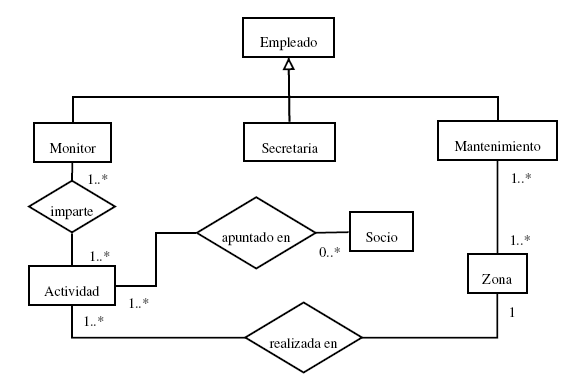
\includegraphics[scale=0.8]{ERe.png}
  \end{center}
  \caption{Diagrama ERe de ejemplo}
\end{figure}


\section{Código fuente}

En \LaTeX tenemos varias maneras de colocar nuestro código fuente, pero
vamos a mostrar dos básicas.

\subsection{Entorno \texttt{Verbatim}}

Este entorno, nos permite incluir dentro de él \negrita{cualquier}
código, y nos respetará espacios, saltos de lineas, tabuladores... es
decir, el compilador de \LaTeX no procesará ese entorno y lo dejará
tal cual está. Veamos un ejemplo con el clásico programa
\programa{Hola mundo} en \texttt{C++}:

\begin{verbatim}
/*Clásico programa en su versión C++*/

#include <iostream>

using namespace std;

int main()
{
  cout << "¡Hola, mundo!" << endl;
  return 0; //No hace falta, pero en fin
}
\end{verbatim}

Vemos, que queda un poco ``soso'': no remarca palabras del lenguaje,
le da igual lo que es comentario y lo que es texto, y claro, a la hora
de tener un código relativamente amplio, pues es incomodo verlo tan
plano. Hay alternativas como \texttt{fncyverbatim}, en la cual podemos
formatearlo algo, añadiendo números de lineas, remarcando palabras del
lenguaje y más opciones, pero quizás la siguiente opción sea más
completa:

\subsection{Entorno \texttt{listing}}

Si vemos en el fichero \comando{comandos.sty}, podemos ver varios
estilos definidos para este entorno. ¿En qué consiste? Pues realmente
este entorno, sabiendo de que lenguaje le estamos pasando el código
(admitiendo gran variedad como C, C++, Java, \TeX, SQL, ADA, Python y
muchísimos más), y ciertas opciones, podemos formatear el código.\\

Este entorno podemos llamarlo de dos formas distintas, la primera es
utilizando un entorno propiamente dicho, con sus
$\backslash$\texttt{begin} y $\backslash$\texttt{end} dentro del cual
copiamos el código, y otra usando el comando
$\backslash$\texttt{lstinputlisting}, pasándole de parámetro el propio
fichero. Veamos de las dos formas:

\begin{lstlisting}[style=C++]
/*Clasico programa en su version C++*/

#include <iostream>

using namespace std;

int main()
{
  cout << "Hola, mundo!" << endl;
  return 0; //No hace falta, pero en fin
}  
\end{lstlisting}

O de la segunda forma:

\lstinputlisting[style=C++]{hola_mundo.cpp}

Notar que uso el estilo \texttt{C++} porque ya lo tengo definido en el
fichero mencionado anteriormente, pero se pueden añadir varios más,
modificando los colores, si queremos o no número de lineas, o por
ejemplo comandos de consola:

\begin{lstlisting}[style=consola]
  g++ hola_mundo.cpp -o hola_mundo
\end{lstlisting}

Desde luego, es bastante más agradable para la vista, lo cual facilita
si lectura. Sin embargo, si usamos esta última opción probablemente
tengamos problemas con los caracteres españoles, acentos y demás,
debido a las diferencias de codificación entre ISO Latin-1 y UTF8. Hay
que tener cuidado en tenerlo todo en UTF8 para que el compilador
``entienda'' los caracteres.

\chapter{Herramientas utilizadas}
% -*-cap2.tex-*-
% Este fichero es parte de la plantilla LaTeX para
% la realización de Proyectos Final de Carrera, protejido
% bajo los términos de la licencia GFDL.
% Para más información, la licencia completa viene incluida en el
% fichero fdl-1.3.tex

% Copyright (C) 2009 Pablo Recio Quijano 

A continuación se listarán las herramientas software que se han usado durante la realización del proyecto, excluyendo aquellas que ya se nombraron y detallaron en los apartados:

\begin{itemize}
\item 5.2. Arquitectura lógica del sistema
\item 6.2. Entorno de construcción
\end{itemize}

\section{Cliente del sistema de control de versiones}

Como ya se comentó anteriormente en el presente documento, el software de control de versiones que se ha usado durante la realización del proyecto ha sido Git, que se integra perfectamente con Android Studio.\\

Aun así, también se ha hecho uso del cliente GitHub para la manipulación del código fuente alojado en el repositorio, así como para versionar ficheros a los que no se accedían directamente desde Android Studio, como por ejemplo aquellos correspondientes a la memoria.

\figura{github.png}{scale=0.6}{Logo de GitHub}{github}{H}

\section{Redacción de la memoria}

Para la completa realización de la memoria se ha usado LATEX. Se trata de un sistema de composición de textos, orientado específicamente a la creación de libros, documentos científicos y técnicos que pudiesen contener fórmulas matemáticas.\\

\figura{latex.png}{scale=0.6}{Logo de LATEX}{latex}{H}

LATEX es un sistema de composición de textos que está formado mayoritariamente por órdenes (mácros) construidas a partir de comandos de TEX. LATEX es una herramienta práctica y útil pues, a su facilidad de uso, se une toda la potencia de TEX.

\section{Gestión del proyecto}

Gatt Project es un programa gratuito multiplataforma desarrollado en Java y especializado en la gestión de proyectos.

\figura{ganttproject.png}{scale=0.6}{Logo de Gantt Project}{ganttproject}{H}

Cuenta con la posibilidad de generar fácilmente diagramas de Gantt para la gestión de los tiempos de las tareas de un proyecti, y gestión de recursos usando gráficos de carga de los mismos. Es muy usado gracias a sus numerosas opciones de reportes (MS Project, HTML, PDF, hojas de cálculo, etc).

\section{Realización de diagramas}

Para la realización de todos los diagramas necesarios que aparecen a lo largo de toda la memoria se ha usado el creador de diagramas llamado Dia.\\

\figura{dia.png}{scale=0.6}{Logo de Dia}{dia}{H}

Dia es un programa de creación de diagramas en GNU/Linux, MacOS X, Unix y Windows, bajo licencia GPL. Puede ser utilizado para dibujar diferentes tipos de diagramas. Actualmente cuenta con herramientas para dibujar diagramas entidad-relación, diagramas UML, diagramas de flujo, diagramas de red y muchos otros tipos.

\section{Ilustración y retoque}

Para la ilustración y retoque de imágenes se ha usado GIMP. GIMP es un programa libre y gratuito de edición de imágenes digitales en forma de mapa de bits. Forma parte del proyecto GNU y está disponible bajo la licencia pública general de GNU. Su interfaz está disponible en varios idiomas.

\figura{gimp.png}{scale=0.6}{Logo de Gimp}{gimp}{H}

En una gran cantidad de casos, GIMP es una alternativa sólida, potente y rápida a Photoshop, aunque no ha sido desarrollado como un clon de éste y por tanto posee una interfaz diferente. Con él se han realizado iconos, botones y edición y retoque de algunos de los recursos usados en la aplicación y en la memoria.


\chapter{Manual de instalación}
% -*-cap2.tex-*-
% Este fichero es parte de la plantilla LaTeX para
% la realización de Proyectos Final de Carrera, protejido
% bajo los términos de la licencia GFDL.
% Para más información, la licencia completa viene incluida en el
% fichero fdl-1.3.tex

% Copyright (C) 2009 Pablo Recio Quijano 


Dado que la aplicación no se encuentra publicada actualmente en Google Play Store, se ha subido el paquete APK con la versión más reciente de la aplicación al repositorio GitHub que se ha usado durante el desarrollo del proyecto.\\

Para descargarlo, basta con que se acceda a la siguiente URL y se pulse sobre el paquete SeniorFitness.apk:\\

\url{https://github.com/alvarogonzalezalvarez/SeniorFitness/tree/master/apk}\\

Es posible que para la instalación del APK en el dispositivo móvil sea necesario activar la opción que permite la instalación de aplicaciones de origen desconocido, lo cual se puede hacer desde los ajustes del sistema del dispositivo móvil usado.


\chapter{Manual de usuario}
% -*-cap2.tex-*-
% Este fichero es parte de la plantilla LaTeX para
% la realización de Proyectos Final de Carrera, protejido
% bajo los términos de la licencia GFDL.
% Para más información, la licencia completa viene incluida en el
% fichero fdl-1.3.tex

% Copyright (C) 2009 Pablo Recio Quijano 


Este capitulo contiene un manual detallado sobre cómo usar la aplicación desarrollada.

\section{Consideraciones previas}

Esta aplicación requiere que la versión de Android instalada en el dispositivo sea igual o superior a la versión 4.0.3. La versión de Android puede ser consultada desde Ajustes -> Información del teléfono -> Versión de Android.

\section{Primera ejecución}

Al instalar y abrir la aplicación por primera vez y por tanto no haber ninguna persona dada de alta en la aplicación, no será posible hacer uso de ninguna de las funcionalidades de la misma, por lo que el primer paso será dar alta a una persona mayor en la aplicación.

\section{Alta de persona}

Todos los campos de la pantalla deben ser cumplimentados obligatoriamente excepto la foto, que se puede dejar sin informar si así se desea. Una vez introducidos, se debe pulsar sobre el botón GUARDAR para que la persona quede dada de alta en la aplicación y se muestre de nuevo la pantalla inicial, mostrando la persona recién registrada. El texto introducido en el campo DNI debe tener un formato de DNI válido.

\subsection{Agregar foto}

Durante el alta de una persona en el sistema, existe la opción de agregar una foto que quedará asociada a la persona, y que será la que se muestre junto a la información de la misma. Para ello es necesario pulsar sobre el botón AGREGAR FOTO, y seguidamente seleccionar una de las dos opciones que se muestran:

\begin{itemize}
\item Tomar foto: Esta opción abre la cámara del dispositivo y permite tomar una fotografía. Una vez tomada, se abrirá la pantalla de edición de imagen para que se pueda seleccionar la sección de la imagen que interese recortar con una relación de aspecto definida por defecto.
\item Seleccionar foto: Esta opción mostrará el explorador de archivos del dispositivo para que se seleccione la foto que se quiera asociar a la persona que se está dando de alta. Al igual que para la opción anterior, se abrirá la pantalla de edición para que se recorte la sección deseada de la imagen.
\end{itemize}

\section{Empezar o continuar con sesión}

Una vez existe al menos una persona dada de alta en la aplicación, ya será posible realizar una sesión de tests. Para ello, desde la pantalla principal, debe pulsarse sobre el icono de las pesas, situado en la esquina superior derecha de la pantalla. Una vez se haya pulsado sobre dicho icono, aparecerá el listado de personas dadas de alta en la aplicación para que se seleccione aquella que iniciará o continuará la sesión.\\

Al seleccionar la persona, se mostrará el listado de tests asociados a la sesión que la persona tenga en progreso en ese momento. En caso de que no tuviese ninguna sesión en progreso, se creará una nueva y se listarán los tests para la misma (al ser una sesión nueva, todos ellos sin realizar). El siguiente paso será seleccionar el test que se quiera llevar a cabo de la batería de pruebas Senior Fitness Test.

\section{Selección de test}

El siguiente paso consiste en seleccionar el test que se quiera realizar de entre los que no se hayan completado aún.  Al lado de cada test se mostrará un icono de información que explicará en que consiste cada prueba y cómo ha de realizarse. Los tests listados en la aplicación son los siguientes: 

\subsection{Fuerza de piernas}

\subsubsection{En qué consiste}

Número de veces que es capaz de sentarse y levantarse de una silla durante un tiempo definido (30 segundos por defecto) con los brazos en cruz y colocados sobre el pecho.

\subsubsection{Uso de la aplicación}

\begin{enumerate}
\item Definir el tiempo que durará el ejercicio (por defecto 30 segundos). 
\item Colocar el dispositivo móvil sobre el muslo de la persona que realiza la prueba. Debe quedar colocado con la pantalla hacia arriba y de forma que sea legible por la persona cuando ésta se encuentra en el punto de partida del ejercicio, esto es, estando sentada. En la siguiente imagen se ilustra como debe quedar colocado el dispositivo en la pierna:

\figura{dispositivo_movil_piernas.png}{scale=0.6}{Colocación del dispositivo móvil para el test Fuerza de piernas}{dispositivo_movil_piernas_instrucciones}{H}
\item Pulsar sobre el botón START.
\item Realizar el ejercicio hasta que termine la cuenta atrás y el dispositivo móvil emita un doble tono de notificación.
\item Pulsar sobre GUARDAR en caso de que se desee registrar el resultado.
\end{enumerate}

\subsection{Fuerza de brazos}

\subsubsection{En qué consiste}

Número de flexiones de brazo completas, sentado en una silla, que realiza durante un tiempo definido (30 segundos por defecto) sujetando una pesa de 3 libras (2,27 kg) para mujeres y 5 libras (3,63 kg) para hombres.

\subsubsection{Uso de la aplicación}

\begin{enumerate}
\item Definir el tiempo que durará el ejercicio (por defecto 30 segundos). 
\item Colocar el dispositivo móvil sobre el antebrazo de la persona que realiza la prueba. Quedará colocado con la pantalla hacia arriba y de forma que sea legible por la persona cuando ésta se encuentra en el punto de partida del ejercicio, esto es, con el brazo extendido. En la siguiente imagen se ilustra la colocación del dispositivo móvil en el brazo de la persona que realizará el ejercicio:

\figura{dispositivo_movil_brazos.png}{scale=0.6}{Colocación del dispositivo móvil para el test Fuerza de brazos}{dispositivo_movil_brazos_instrucciones}{H}

\item Pulsar sobre el botón START.
\item Realizar el ejercicio hasta que termine la cuenta atrás y el dispositivo móvil emita un doble tono de notificación.
\item Pulsar sobre GUARDAR en caso de que se desee registrar el resultado.
\end{enumerate}

\subsection{Resistencia aeróbica}

\subsubsection{En qué consiste}

Número de veces que levanta la rodilla hasta una altura equivalente al punto medio entre la rótula y la cresta ilíaca durante un tiempo definido (2 minutos por defecto). Se contabiliza una vez por cada ciclo (derecha-izquierda).

\subsubsection{Uso de la aplicación}

\begin{enumerate}
\item Definir el tiempo que durará el ejercicio (por defecto 120 segundos). 
\item Colocar el dispositivo móvil sobre el muslo de la persona que realiza la prueba. Debe quedar colocado con la pantalla hacia arriba y de forma que sea legible por la persona cuando ésta se encuentra en el punto de partida del ejercicio, esto es, estando sentada. En la siguiente imagen se ilustra como debe quedar colocado el dispositivo en la pierna:

\figura{dispositivo_movil_piernas.png}{scale=0.6}{Colocación del dispositivo móvil para el test Fuerza de piernas}{dispositivo_movil_resistencia_instrucciones}{H}
\item Pulsar sobre el botón START.
\item Realizar el ejercicio hasta que termine la cuenta atrás y el dispositivo móvil emita un doble tono de notificación.
\item Pulsar sobre GUARDAR en caso de que se desee registrar el resultado.
\end{enumerate}

\subsection{Flexibilidad de piernas}

\subsubsection{En qué consiste}

Sentado en el borde de una silla, estirar la pierna y las manos intentan alcanzar los dedos del pie que está con una flexión de tobillo de 90 grados. Se mide la distancia entre la punta de los dedos de la mano y la punta del pie (positiva si los dedos de la mano sobrepasan los dedos del pie o negativa si los dedos de la manos no alcanzan a tocar los dedos del pie).

\subsubsection{Uso de la aplicación}

\begin{enumerate}
\item Introducir en la aplicación la medida obtenida.
\item Pulsar sobre GUARDAR en caso de que se desee registrar el valor introducido.
\end{enumerate}

\subsection{Flexibilidad de brazos}

\subsubsection{En qué consiste}

Una mano se pasa por encima del mismo hombro y la otra pasa a tocar la parte media de la espalda intentando que ambas manos se toquen. Se mide la distancia entre la punta de los dedos de cada mano (positiva si los dedos de la mano se superponen o negativa si no llegan a tocarse los dedos de la mano).

\subsubsection{Uso de la aplicación}

\begin{enumerate}
\item Introducir en la aplicación la medida obtenida.
\item Pulsar sobre GUARDAR en caso de que se desee registrar el valor introducido.
\end{enumerate}

\subsection{Agilidad}

\subsubsection{En qué consiste}

Partiendo de sentado, tiempo que tarda en levantarse caminar hasta un cono situado a 2,44 metros, girar y volver a sentarse.

\subsubsection{Uso de la aplicación}

\begin{enumerate}
\item Pulsar sobre el botón START cuando se vaya a iniciar el ejercicio.
\item Pulsar sobre el botón STOP cuando la persona haya vuelto a sentarse tras completar el ejercicio.
\item Pulsar sobre GUARDAR en caso de que se desee registrar el tiempo obtenido.
\end{enumerate}

\section{Consultar detalle e historial de persona}

Si se desea consultar el perfil de una persona dada de alta en la aplicación, basta con pulsar sobre ella en la pantalla principal. Se abrirá entonces la pantalla que muestra el detalle de la persona, donde se podrán realizar las siguientes acciones:

\begin{itemize}
\item Eliminar persona: Si se desea eliminar de la aplicación a la persona seleccionada, basta con pulsar sobre el icono de la papelera, situado en la esquina superior derecha de la pantalla, y confirmar la acción.
\item Consultar sesiones ya realizadas: Si se desea consultar las estadísticas de una sesión ya realizada, basta con pulsar sobre cualquier sesión completada para que se muestre el detalle de la misma.
\item Continuar sesión en progreso: Si la persona dispone de una sesión en progreso y se pulsa sobre ella, se cargará la pantalla de selección de test y se podrá continuar con la sesión desde el estado en el que se encontraba.
\end{itemize}

\chapter{Conclusiones}
% -*-cap2.tex-*-
% Este fichero es parte de la plantilla LaTeX para
% la realización de Proyectos Final de Carrera, protejido
% bajo los términos de la licencia GFDL.
% Para más información, la licencia completa viene incluida en el
% fichero fdl-1.3.tex

% Copyright (C) 2009 Pablo Recio Quijano 

En este capítulo se detallan los objetivos alcanzados, las enseñanzas obtenidas por parte del desarrollador del proyecto y las posibles mejoras futuras que puedan implementarse en el sistema.

\section{Objetivos alcanzados}

A pesar de que a lo largo del desarrollo del proyecto han ido surgiendo nuevas ideas y cambios con respecto a los planteamientos iniciales, podemos concluir que se han conseguido alcanzar los objetivos principales y las ideas base que se definieron durante la definición de la aplicación, dado que ésta nos permite de forma sencilla llevar un control y seguimiento sobre la condición física funcional de personas mayores, siempre basándonos en las pruebas y criterios definidos en la batería de pruebas Senior Fitness Test.\\

\section{Lecciones aprendidas}

Durante el desarrollo del proyecto he podido adquirir nuevos conocimientos y refrescar otros tantos que estudié durante la realización de la carrera años atrás y que, debido a que las metodologías de trabajo actualmente están en constante evolución en el mundo laboral y que éstas se van adaptando a las necesidades de la empresa, no había tenido ocasión de poner en práctica. Algunos ejemplos podrían ser la realización de los diagramas de secuencia y otros conceptos relacionados con UML.\\

Es importante destacar también que es la primera vez que me enfrento al desarrollo de una aplicación móvil Android completa. Anteriormente había realizado de forma autodidacta pequeños tutoriales y ejercicios, pero no ha sido hasta la realización de este proyecto cuando he podido obtener y consolidar los conocimientos necesarios para, desde 0, crear una aplicación haciendo uso de Android.\\

Por otro lado también me gustaría dejar constancia de todo lo que me llevo aprendido en relación al tema que abarca el proyecto, lo cual me ha llevado a tener que indagar sobre el mundo e-health para contextualizar el uso y la finalidad principal de la aplicación.\\

En definitiva, puedo concluir que el afrontar este proyecto ha supuesto un reto tanto personal como intelectual.

\section{Trabajo futuro}

A lo largo del desarrollo del proyecto se han barajado ciertas opciones o alternativas que, al no haber sido implementadas en la versión actual de la aplicación, podrían ser aplicadas en futuras versiones o mejoras que se añadan al proyecto. Además, es indispensable contar con el hecho de que aparecerán posibles ampliaciones futuras en cada una de las facetas en las que se divide el sistema. A continuación listamos algunas:

\begin{itemize}
\item Estudiar la posibilidad de que, para los tests de flexibilidad de brazos y flexibilidad de piernas, a través de la cámara o de algún sensor de proximidad del dispositivo, se pueda obtener la distancia de separación entre los dedos de la mano con respecto a la punta del pie para el caso del test de flexibilidad de piernas, o la distancia de separación entre los dedos de ambas manos para el caso del test de flexibilidad de brazos.
\item Para el test de Agilidad, estudiar la posibilidad de añadir un contador de pasos que, a través del dispositivo, calcule aproximadamente la distancia recorrida y la persona sepa cuando volver hacia su sitio sin necesidad de colocar un cono a una distancia determinada.
\item Añadir un selector de sesiones completadas que permita seleccionar las que se deseen para comparar entre las mismas los resultados obtenidos en cada una de ellas.
\item En la pantalla de información de los tests que hacen uso del dispositivo para detectar el movimiento, añadir un botón que permita hacer una prueba del movimiento requerido para comprobar que la persona se familiariza con el mismo antes de realizar el test.
\item Actualmente el APK de la aplicación se encuentra disponible para su descarga en el repositorio GitHub ya mencionado en el presente documento. Sería interesante publicar la aplicación en Google Play Store para facilitar su instalación y distribución.
\item La interfaz gráfica de la aplicación se encuentra en español. Para futuras líneas de actuación del proyecto sería interesante que el sistema estuviera disponible en otros idiomas, como por ejemplo en inglés.
\end{itemize}




\backmatter % Apéndices, bibliografia ...


\clearpage
\addcontentsline{toc}{chapter}{Bibliografia y referencias}
\bibliographystyle{unsrt}
\bibliography{bibliografia}


% This is set up to run with pdflatex.
%---------The file header---------------------------------------------
%---------------------------------------------------------------------
\chapter*{\rlap{GNU Free Documentation License}}
\phantomsection  % so hyperref creates bookmarks
\addcontentsline{toc}{chapter}{GNU Free Documentation License}
%\label{label_fdl}

 \begin{center}

       Version 1.3, 3 November 2008


 Copyright \copyright{} 2000, 2001, 2002, 2007, 2008  Free Software Foundation, Inc.
 
 \bigskip
 
     <http://fsf.org/>
  
 \bigskip
 
 Everyone is permitted to copy and distribute verbatim copies
 of this license document, but changing it is not allowed.
\end{center}


\begin{center}
{\bf\large Preamble}
\end{center}

The purpose of this License is to make a manual, textbook, or other
functional and useful document ``free'' in the sense of freedom: to
assure everyone the effective freedom to copy and redistribute it,
with or without modifying it, either commercially or noncommercially.
Secondarily, this License preserves for the author and publisher a way
to get credit for their work, while not being considered responsible
for modifications made by others.

This License is a kind of ``copyleft'', which means that derivative
works of the document must themselves be free in the same sense.  It
complements the GNU General Public License, which is a copyleft
license designed for free software.

We have designed this License in order to use it for manuals for free
software, because free software needs free documentation: a free
program should come with manuals providing the same freedoms that the
software does.  But this License is not limited to software manuals;
it can be used for any textual work, regardless of subject matter or
whether it is published as a printed book.  We recommend this License
principally for works whose purpose is instruction or reference.


\begin{center}
{\Large\bf 1. APPLICABILITY AND DEFINITIONS\par}
\phantomsection
\addcontentsline{toc}{section}{1. APPLICABILITY AND DEFINITIONS}
\end{center}

This License applies to any manual or other work, in any medium, that
contains a notice placed by the copyright holder saying it can be
distributed under the terms of this License.  Such a notice grants a
world-wide, royalty-free license, unlimited in duration, to use that
work under the conditions stated herein.  The ``\textbf{Document}'', below,
refers to any such manual or work.  Any member of the public is a
licensee, and is addressed as ``\textbf{you}''.  You accept the license if you
copy, modify or distribute the work in a way requiring permission
under copyright law.

A ``\textbf{Modified Version}'' of the Document means any work containing the
Document or a portion of it, either copied verbatim, or with
modifications and/or translated into another language.

A ``\textbf{Secondary Section}'' is a named appendix or a front-matter section of
the Document that deals exclusively with the relationship of the
publishers or authors of the Document to the Document's overall subject
(or to related matters) and contains nothing that could fall directly
within that overall subject.  (Thus, if the Document is in part a
textbook of mathematics, a Secondary Section may not explain any
mathematics.)  The relationship could be a matter of historical
connection with the subject or with related matters, or of legal,
commercial, philosophical, ethical or political position regarding
them.

The ``\textbf{Invariant Sections}'' are certain Secondary Sections whose titles
are designated, as being those of Invariant Sections, in the notice
that says that the Document is released under this License.  If a
section does not fit the above definition of Secondary then it is not
allowed to be designated as Invariant.  The Document may contain zero
Invariant Sections.  If the Document does not identify any Invariant
Sections then there are none.

The ``\textbf{Cover Texts}'' are certain short passages of text that are listed,
as Front-Cover Texts or Back-Cover Texts, in the notice that says that
the Document is released under this License.  A Front-Cover Text may
be at most 5 words, and a Back-Cover Text may be at most 25 words.

A ``\textbf{Transparent}'' copy of the Document means a machine-readable copy,
represented in a format whose specification is available to the
general public, that is suitable for revising the document
straightforwardly with generic text editors or (for images composed of
pixels) generic paint programs or (for drawings) some widely available
drawing editor, and that is suitable for input to text formatters or
for automatic translation to a variety of formats suitable for input
to text formatters.  A copy made in an otherwise Transparent file
format whose markup, or absence of markup, has been arranged to thwart
or discourage subsequent modification by readers is not Transparent.
An image format is not Transparent if used for any substantial amount
of text.  A copy that is not ``Transparent'' is called ``\textbf{Opaque}''.

Examples of suitable formats for Transparent copies include plain
ASCII without markup, Texinfo input format, LaTeX input format, SGML
or XML using a publicly available DTD, and standard-conforming simple
HTML, PostScript or PDF designed for human modification.  Examples of
transparent image formats include PNG, XCF and JPG.  Opaque formats
include proprietary formats that can be read and edited only by
proprietary word processors, SGML or XML for which the DTD and/or
processing tools are not generally available, and the
machine-generated HTML, PostScript or PDF produced by some word
processors for output purposes only.

The ``\textbf{Title Page}'' means, for a printed book, the title page itself,
plus such following pages as are needed to hold, legibly, the material
this License requires to appear in the title page.  For works in
formats which do not have any title page as such, ``Title Page'' means
the text near the most prominent appearance of the work's title,
preceding the beginning of the body of the text.

The ``\textbf{publisher}'' means any person or entity that distributes
copies of the Document to the public.

A section ``\textbf{Entitled XYZ}'' means a named subunit of the Document whose
title either is precisely XYZ or contains XYZ in parentheses following
text that translates XYZ in another language.  (Here XYZ stands for a
specific section name mentioned below, such as ``\textbf{Acknowledgements}'',
``\textbf{Dedications}'', ``\textbf{Endorsements}'', or ``\textbf{History}''.)  
To ``\textbf{Preserve the Title}''
of such a section when you modify the Document means that it remains a
section ``Entitled XYZ'' according to this definition.

The Document may include Warranty Disclaimers next to the notice which
states that this License applies to the Document.  These Warranty
Disclaimers are considered to be included by reference in this
License, but only as regards disclaiming warranties: any other
implication that these Warranty Disclaimers may have is void and has
no effect on the meaning of this License.


\begin{center}
{\Large\bf 2. VERBATIM COPYING\par}
\phantomsection
\addcontentsline{toc}{section}{2. VERBATIM COPYING}
\end{center}

You may copy and distribute the Document in any medium, either
commercially or noncommercially, provided that this License, the
copyright notices, and the license notice saying this License applies
to the Document are reproduced in all copies, and that you add no other
conditions whatsoever to those of this License.  You may not use
technical measures to obstruct or control the reading or further
copying of the copies you make or distribute.  However, you may accept
compensation in exchange for copies.  If you distribute a large enough
number of copies you must also follow the conditions in section~3.

You may also lend copies, under the same conditions stated above, and
you may publicly display copies.


\begin{center}
{\Large\bf 3. COPYING IN QUANTITY\par}
\phantomsection
\addcontentsline{toc}{section}{3. COPYING IN QUANTITY}
\end{center}


If you publish printed copies (or copies in media that commonly have
printed covers) of the Document, numbering more than 100, and the
Document's license notice requires Cover Texts, you must enclose the
copies in covers that carry, clearly and legibly, all these Cover
Texts: Front-Cover Texts on the front cover, and Back-Cover Texts on
the back cover.  Both covers must also clearly and legibly identify
you as the publisher of these copies.  The front cover must present
the full title with all words of the title equally prominent and
visible.  You may add other material on the covers in addition.
Copying with changes limited to the covers, as long as they preserve
the title of the Document and satisfy these conditions, can be treated
as verbatim copying in other respects.

If the required texts for either cover are too voluminous to fit
legibly, you should put the first ones listed (as many as fit
reasonably) on the actual cover, and continue the rest onto adjacent
pages.

If you publish or distribute Opaque copies of the Document numbering
more than 100, you must either include a machine-readable Transparent
copy along with each Opaque copy, or state in or with each Opaque copy
a computer-network location from which the general network-using
public has access to download using public-standard network protocols
a complete Transparent copy of the Document, free of added material.
If you use the latter option, you must take reasonably prudent steps,
when you begin distribution of Opaque copies in quantity, to ensure
that this Transparent copy will remain thus accessible at the stated
location until at least one year after the last time you distribute an
Opaque copy (directly or through your agents or retailers) of that
edition to the public.

It is requested, but not required, that you contact the authors of the
Document well before redistributing any large number of copies, to give
them a chance to provide you with an updated version of the Document.


\begin{center}
{\Large\bf 4. MODIFICATIONS\par}
\phantomsection
\addcontentsline{toc}{section}{4. MODIFICATIONS}
\end{center}

You may copy and distribute a Modified Version of the Document under
the conditions of sections 2 and 3 above, provided that you release
the Modified Version under precisely this License, with the Modified
Version filling the role of the Document, thus licensing distribution
and modification of the Modified Version to whoever possesses a copy
of it.  In addition, you must do these things in the Modified Version:

\begin{itemize}
\item[A.] 
   Use in the Title Page (and on the covers, if any) a title distinct
   from that of the Document, and from those of previous versions
   (which should, if there were any, be listed in the History section
   of the Document).  You may use the same title as a previous version
   if the original publisher of that version gives permission.
   
\item[B.]
   List on the Title Page, as authors, one or more persons or entities
   responsible for authorship of the modifications in the Modified
   Version, together with at least five of the principal authors of the
   Document (all of its principal authors, if it has fewer than five),
   unless they release you from this requirement.
   
\item[C.]
   State on the Title page the name of the publisher of the
   Modified Version, as the publisher.
   
\item[D.]
   Preserve all the copyright notices of the Document.
   
\item[E.]
   Add an appropriate copyright notice for your modifications
   adjacent to the other copyright notices.
   
\item[F.]
   Include, immediately after the copyright notices, a license notice
   giving the public permission to use the Modified Version under the
   terms of this License, in the form shown in the Addendum below.
   
\item[G.]
   Preserve in that license notice the full lists of Invariant Sections
   and required Cover Texts given in the Document's license notice.
   
\item[H.]
   Include an unaltered copy of this License.
   
\item[I.]
   Preserve the section Entitled ``History'', Preserve its Title, and add
   to it an item stating at least the title, year, new authors, and
   publisher of the Modified Version as given on the Title Page.  If
   there is no section Entitled ``History'' in the Document, create one
   stating the title, year, authors, and publisher of the Document as
   given on its Title Page, then add an item describing the Modified
   Version as stated in the previous sentence.
   
\item[J.]
   Preserve the network location, if any, given in the Document for
   public access to a Transparent copy of the Document, and likewise
   the network locations given in the Document for previous versions
   it was based on.  These may be placed in the ``History'' section.
   You may omit a network location for a work that was published at
   least four years before the Document itself, or if the original
   publisher of the version it refers to gives permission.
   
\item[K.]
   For any section Entitled ``Acknowledgements'' or ``Dedications'',
   Preserve the Title of the section, and preserve in the section all
   the substance and tone of each of the contributor acknowledgements
   and/or dedications given therein.
   
\item[L.]
   Preserve all the Invariant Sections of the Document,
   unaltered in their text and in their titles.  Section numbers
   or the equivalent are not considered part of the section titles.
   
\item[M.]
   Delete any section Entitled ``Endorsements''.  Such a section
   may not be included in the Modified Version.
   
\item[N.]
   Do not retitle any existing section to be Entitled ``Endorsements''
   or to conflict in title with any Invariant Section.
   
\item[O.]
   Preserve any Warranty Disclaimers.
\end{itemize}

If the Modified Version includes new front-matter sections or
appendices that qualify as Secondary Sections and contain no material
copied from the Document, you may at your option designate some or all
of these sections as invariant.  To do this, add their titles to the
list of Invariant Sections in the Modified Version's license notice.
These titles must be distinct from any other section titles.

You may add a section Entitled ``Endorsements'', provided it contains
nothing but endorsements of your Modified Version by various
parties---for example, statements of peer review or that the text has
been approved by an organization as the authoritative definition of a
standard.

You may add a passage of up to five words as a Front-Cover Text, and a
passage of up to 25 words as a Back-Cover Text, to the end of the list
of Cover Texts in the Modified Version.  Only one passage of
Front-Cover Text and one of Back-Cover Text may be added by (or
through arrangements made by) any one entity.  If the Document already
includes a cover text for the same cover, previously added by you or
by arrangement made by the same entity you are acting on behalf of,
you may not add another; but you may replace the old one, on explicit
permission from the previous publisher that added the old one.

The author(s) and publisher(s) of the Document do not by this License
give permission to use their names for publicity for or to assert or
imply endorsement of any Modified Version.


\begin{center}
{\Large\bf 5. COMBINING DOCUMENTS\par}
\phantomsection
\addcontentsline{toc}{section}{5. COMBINING DOCUMENTS}
\end{center}


You may combine the Document with other documents released under this
License, under the terms defined in section~4 above for modified
versions, provided that you include in the combination all of the
Invariant Sections of all of the original documents, unmodified, and
list them all as Invariant Sections of your combined work in its
license notice, and that you preserve all their Warranty Disclaimers.

The combined work need only contain one copy of this License, and
multiple identical Invariant Sections may be replaced with a single
copy.  If there are multiple Invariant Sections with the same name but
different contents, make the title of each such section unique by
adding at the end of it, in parentheses, the name of the original
author or publisher of that section if known, or else a unique number.
Make the same adjustment to the section titles in the list of
Invariant Sections in the license notice of the combined work.

In the combination, you must combine any sections Entitled ``History''
in the various original documents, forming one section Entitled
``History''; likewise combine any sections Entitled ``Acknowledgements'',
and any sections Entitled ``Dedications''.  You must delete all sections
Entitled ``Endorsements''.

\begin{center}
{\Large\bf 6. COLLECTIONS OF DOCUMENTS\par}
\phantomsection
\addcontentsline{toc}{section}{6. COLLECTIONS OF DOCUMENTS}
\end{center}

You may make a collection consisting of the Document and other documents
released under this License, and replace the individual copies of this
License in the various documents with a single copy that is included in
the collection, provided that you follow the rules of this License for
verbatim copying of each of the documents in all other respects.

You may extract a single document from such a collection, and distribute
it individually under this License, provided you insert a copy of this
License into the extracted document, and follow this License in all
other respects regarding verbatim copying of that document.


\begin{center}
{\Large\bf 7. AGGREGATION WITH INDEPENDENT WORKS\par}
\phantomsection
\addcontentsline{toc}{section}{7. AGGREGATION WITH INDEPENDENT WORKS}
\end{center}


A compilation of the Document or its derivatives with other separate
and independent documents or works, in or on a volume of a storage or
distribution medium, is called an ``aggregate'' if the copyright
resulting from the compilation is not used to limit the legal rights
of the compilation's users beyond what the individual works permit.
When the Document is included in an aggregate, this License does not
apply to the other works in the aggregate which are not themselves
derivative works of the Document.

If the Cover Text requirement of section~3 is applicable to these
copies of the Document, then if the Document is less than one half of
the entire aggregate, the Document's Cover Texts may be placed on
covers that bracket the Document within the aggregate, or the
electronic equivalent of covers if the Document is in electronic form.
Otherwise they must appear on printed covers that bracket the whole
aggregate.


\begin{center}
{\Large\bf 8. TRANSLATION\par}
\phantomsection
\addcontentsline{toc}{section}{8. TRANSLATION}
\end{center}


Translation is considered a kind of modification, so you may
distribute translations of the Document under the terms of section~4.
Replacing Invariant Sections with translations requires special
permission from their copyright holders, but you may include
translations of some or all Invariant Sections in addition to the
original versions of these Invariant Sections.  You may include a
translation of this License, and all the license notices in the
Document, and any Warranty Disclaimers, provided that you also include
the original English version of this License and the original versions
of those notices and disclaimers.  In case of a disagreement between
the translation and the original version of this License or a notice
or disclaimer, the original version will prevail.

If a section in the Document is Entitled ``Acknowledgements'',
``Dedications'', or ``History'', the requirement (section~4) to Preserve
its Title (section~1) will typically require changing the actual
title.


\begin{center}
{\Large\bf 9. TERMINATION\par}
\phantomsection
\addcontentsline{toc}{section}{9. TERMINATION}
\end{center}


You may not copy, modify, sublicense, or distribute the Document
except as expressly provided under this License.  Any attempt
otherwise to copy, modify, sublicense, or distribute it is void, and
will automatically terminate your rights under this License.

However, if you cease all violation of this License, then your license
from a particular copyright holder is reinstated (a) provisionally,
unless and until the copyright holder explicitly and finally
terminates your license, and (b) permanently, if the copyright holder
fails to notify you of the violation by some reasonable means prior to
60 days after the cessation.

Moreover, your license from a particular copyright holder is
reinstated permanently if the copyright holder notifies you of the
violation by some reasonable means, this is the first time you have
received notice of violation of this License (for any work) from that
copyright holder, and you cure the violation prior to 30 days after
your receipt of the notice.

Termination of your rights under this section does not terminate the
licenses of parties who have received copies or rights from you under
this License.  If your rights have been terminated and not permanently
reinstated, receipt of a copy of some or all of the same material does
not give you any rights to use it.


\begin{center}
{\Large\bf 10. FUTURE REVISIONS OF THIS LICENSE\par}
\phantomsection
\addcontentsline{toc}{section}{10. FUTURE REVISIONS OF THIS LICENSE}
\end{center}


The Free Software Foundation may publish new, revised versions
of the GNU Free Documentation License from time to time.  Such new
versions will be similar in spirit to the present version, but may
differ in detail to address new problems or concerns.  See
http://www.gnu.org/copyleft/.

Each version of the License is given a distinguishing version number.
If the Document specifies that a particular numbered version of this
License ``or any later version'' applies to it, you have the option of
following the terms and conditions either of that specified version or
of any later version that has been published (not as a draft) by the
Free Software Foundation.  If the Document does not specify a version
number of this License, you may choose any version ever published (not
as a draft) by the Free Software Foundation.  If the Document
specifies that a proxy can decide which future versions of this
License can be used, that proxy's public statement of acceptance of a
version permanently authorizes you to choose that version for the
Document.


\begin{center}
{\Large\bf 11. RELICENSING\par}
\phantomsection
\addcontentsline{toc}{section}{11. RELICENSING}
\end{center}


``Massive Multiauthor Collaboration Site'' (or ``MMC Site'') means any
World Wide Web server that publishes copyrightable works and also
provides prominent facilities for anybody to edit those works.  A
public wiki that anybody can edit is an example of such a server.  A
``Massive Multiauthor Collaboration'' (or ``MMC'') contained in the
site means any set of copyrightable works thus published on the MMC
site.

``CC-BY-SA'' means the Creative Commons Attribution-Share Alike 3.0
license published by Creative Commons Corporation, a not-for-profit
corporation with a principal place of business in San Francisco,
California, as well as future copyleft versions of that license
published by that same organization.

``Incorporate'' means to publish or republish a Document, in whole or
in part, as part of another Document.

An MMC is ``eligible for relicensing'' if it is licensed under this
License, and if all works that were first published under this License
somewhere other than this MMC, and subsequently incorporated in whole
or in part into the MMC, (1) had no cover texts or invariant sections,
and (2) were thus incorporated prior to November 1, 2008.

The operator of an MMC Site may republish an MMC contained in the site
under CC-BY-SA on the same site at any time before August 1, 2009,
provided the MMC is eligible for relicensing.


\begin{center}
{\Large\bf ADDENDUM: How to use this License for your documents\par}
\phantomsection
\addcontentsline{toc}{section}{ADDENDUM: How to use this License for your documents}
\end{center}

To use this License in a document you have written, include a copy of
the License in the document and put the following copyright and
license notices just after the title page:

\bigskip
\begin{quote}
    Copyright \copyright{}  YEAR  YOUR NAME.
    Permission is granted to copy, distribute and/or modify this document
    under the terms of the GNU Free Documentation License, Version 1.3
    or any later version published by the Free Software Foundation;
    with no Invariant Sections, no Front-Cover Texts, and no Back-Cover Texts.
    A copy of the license is included in the section entitled ``GNU
    Free Documentation License''.
\end{quote}
\bigskip
    
If you have Invariant Sections, Front-Cover Texts and Back-Cover Texts,
replace the ``with \dots\ Texts.'' line with this:

\bigskip
\begin{quote}
    with the Invariant Sections being LIST THEIR TITLES, with the
    Front-Cover Texts being LIST, and with the Back-Cover Texts being LIST.
\end{quote}
\bigskip
    
If you have Invariant Sections without Cover Texts, or some other
combination of the three, merge those two alternatives to suit the
situation.

If your document contains nontrivial examples of program code, we
recommend releasing these examples in parallel under your choice of
free software license, such as the GNU General Public License,
to permit their use in free software.

%---------------------------------------------------------------------


\end{document}
